\documentclass[dvipdfmx,cjk]{beamer} 
%\documentclass[dvipdfm,cjk]{beamer} %% オプションは環境や利用するプログラムに
%\documentclass[dvips,cjk]{beamer}   %% よって変える

\AtBeginDvi{\special{pdf:tounicode 90ms-RKSJ-UCS2}} %% しおりが文字化けしないように
%\AtBeginDvi{\special{pdf:tounicode EUC-UCS2}}

%\setbeamertemplate{navigation symbols}{} %% 右下のアイコンを消す

%\usetheme{CambridgeUS}         %% theme の選択
%\usetheme{Boadilla}           %% Beamer のディレクトリの中の
\usetheme{Madrid}             %% beamerthemeCambridgeUS.sty を指定
%\usetheme{Antibes}            %% 色々と試してみるといいだろう
%\usetheme{Montpellier}        %% サンプルが beamer\doc に色々とある。
%\usetheme{Berkeley}
%\usetheme{Goettingen}
%\usetheme{Singapore}
%\usetheme{Szeged}

%\usecolortheme{rose}          %% colortheme を選ぶと色使いが変わる
%\usecolortheme{albatross}

%\useoutertheme{shadow}                 %% 箱に影をつける
%\usefonttheme{professionalfonts}       %% 数式の文字を通常の LaTeX と同じにする

%\setbeamercovered{transparent}         %% 消えている文字をうっすらと表示する
\usepackage{bxdpx-beamer}
\usepackage{pxjahyper}
\usepackage{minijs}
\usepackage{mathrsfs}
\usepackage{amsmath,amsfonts,amsthm,amssymb}
\usepackage{color}
\usepackage{graphics}
\usepackage{tikz}
\usepackage{bm,bbm}
\usepackage{picture}
\usepackage{fancybox}
\usepackage[bold]{otf}
\usepackage{here}
%定理環境の設定
%\usepackage{amsthm}
\theoremstyle{definition}
%\setbeamertemplate{theorems}[numbered] % 定理などに番号をふるために必要 %
\newtheorem{rem}{\textbf{ 注意 }}
\newtheorem{ex}{\textbf{ 例 }}
\newtheorem{dfn}{\textbf{ 定義 }}
\newtheorem{thm}[dfn]{\textbf{ 定理 }}
\newtheorem{prop}[dfn]{\textbf{ 命題 }}
\newtheorem{lem}[dfn]{\textbf{ 補題 }}
\newtheorem{cor}[dfn]{\textbf{ 系 }}
\newtheorem{axi}[dfn]{\textbf{ 公理 }}
\renewcommand{\proofname}{\textbf{証明}}




%スタイルファイルを追加したい場合は以下のように書く
\usepackage{graphicx}
\usepackage{amsmath,amssymb}
%\usepackage{eclbkbox}
\usepackage{tikz}

%\newcommandでマクロを定義できる
\newcommand{\macrotest}{\LaTeX のマクロは便利}
\newcommand{\PD}[2]{\frac{\partial {#1}}{\partial {#2}}}%引数もとれる
\newcommand{\combination}[2]{{}_{#1} \mathrm{C}_{#2}}

\begin{document}
\title[多様体の次元を調べる方法]{多様体の次元を調べる方法} 
\author[青見健志]{青見健志}            %% ここに書かれた情報は色々なところに使われるので
\institute[空間数理研究室]{空間数理研究室}   %% なるべく設定した方が良い
\date{令和6年2月8日}

\begin{frame}                  %% \begin{frame}..\end{frame} で 1 枚のスライド
\titlepage                     %% タイトルページ
\end{frame}

\begin{frame}                  %% 目次 (必要なければ省略)
\tableofcontents
\end{frame}

\section{はじめに}
\begin{frame}
\frametitle{はじめに} 
どこでも好きなところに$m$次元の局所座標系
を描ける空間を$m$次元多様体という. 例えば, 球面
は球面上のどこでも好きなところに
$2$次元の局所座標系を描くことができるため, 
$2$次元多様体である.  

私は空間の多様体としての
次元を調べることで複雑な方程式で表された空間や
高次元の空間などの形を理解できることに興味をもち, 
多様体の次元を調べる方法を研究することにした. 
  \begin{figure}[]
    \centering
    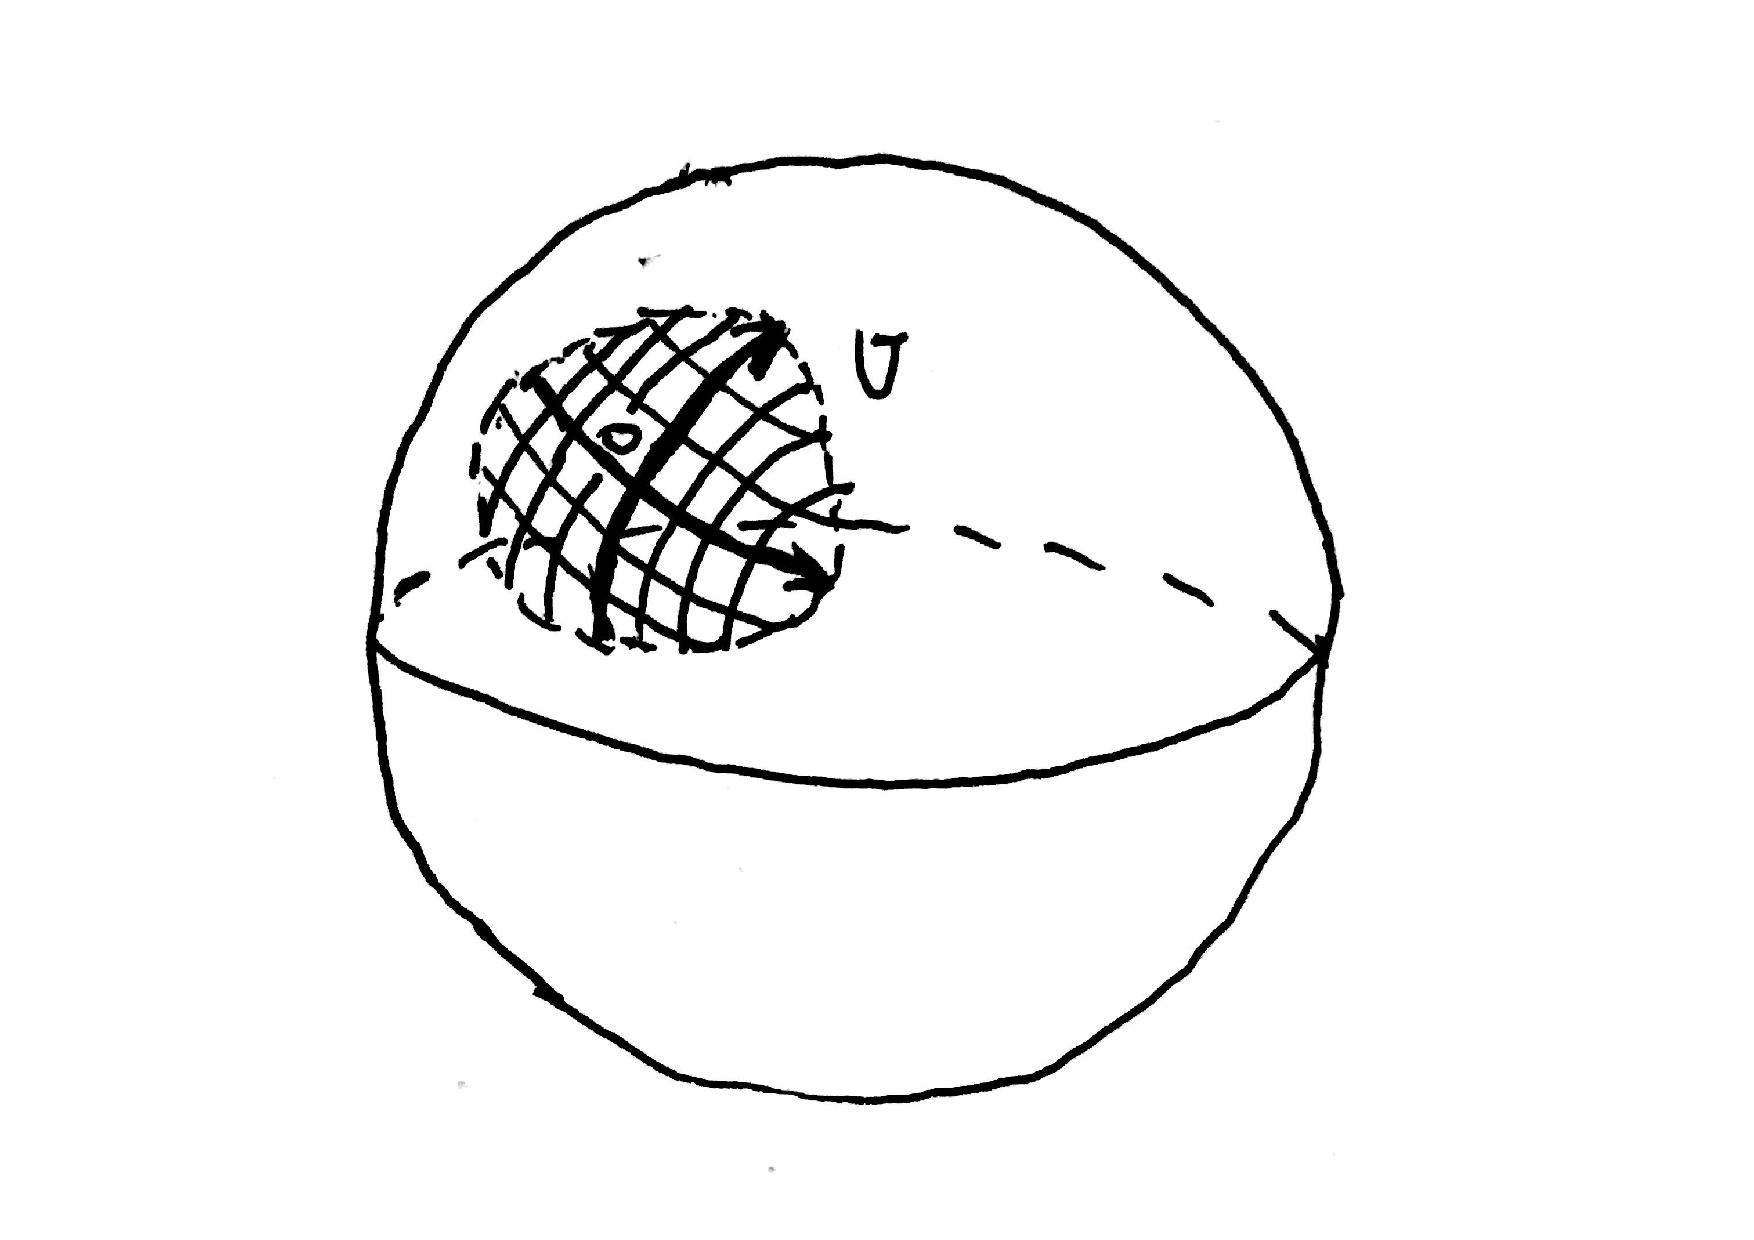
\includegraphics[keepaspectratio, scale=0.2]
         {CoSysInS2.pdf}
    \caption{球面に描かれた局所座標系}
    \label{CoSysInS2}
   \end{figure}
\end{frame}

\section{準備}
\begin{frame}
\frametitle{準備} 
\begin{dfn}
位相空間$X$の開集合$U$から, $m$次元数空間$\mathbb{R}^m$のある開集合$U'$
への同相写像
$\varphi : U\rightarrow U'$
があるとき$\varphi$を$U$上の局所座標系といい, 
$(U, \varphi)$を$m$次元座標近傍という. 

\end{dfn}
\begin{figure}[H]
  \begin{tabular}{cc}
    %---- 最初の図 ---------------------------
    \begin{minipage}[t]{0.45\hsize}
      \centering
      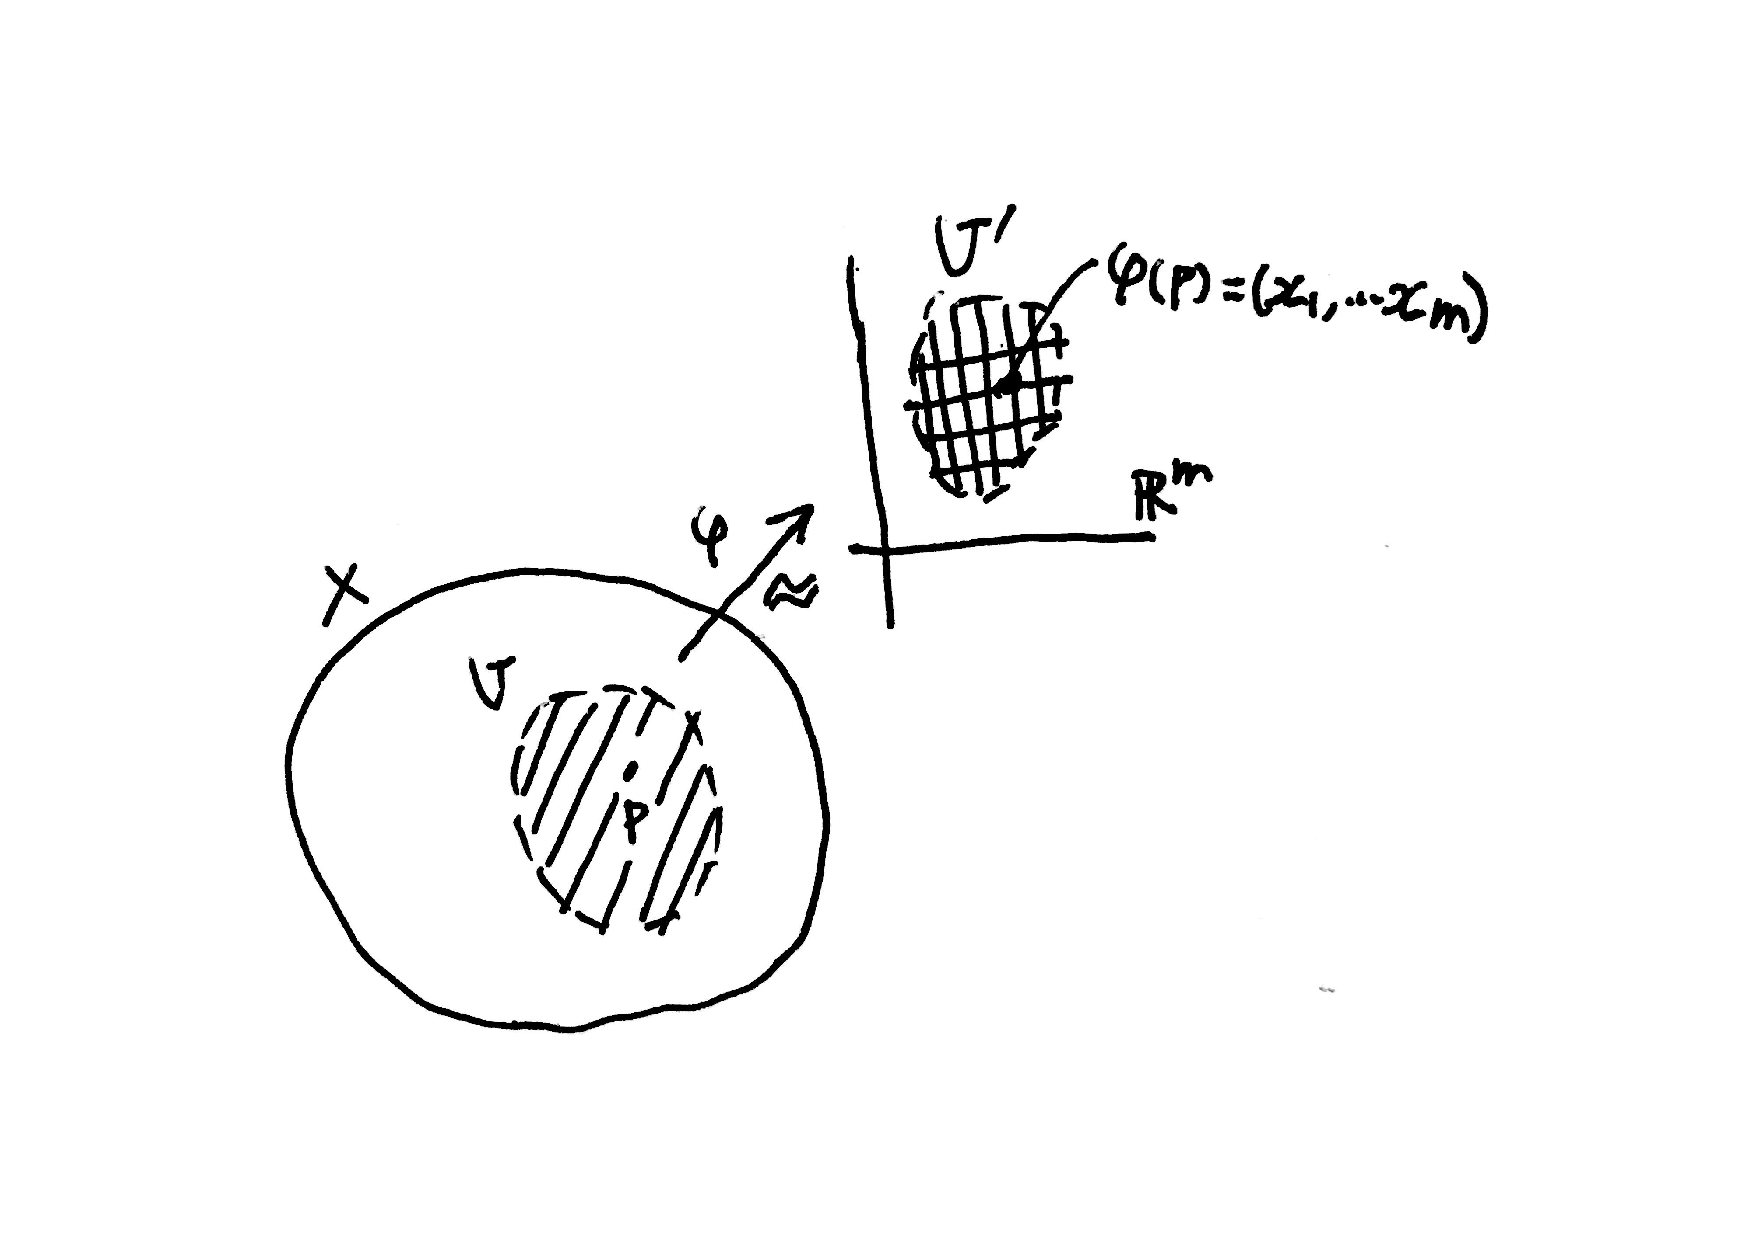
\includegraphics[keepaspectratio, scale=0.2]{coNeighborhoodBig.pdf}
      \caption{$U$上の局所座標系}
      \label{}
    \end{minipage} &
    %---- 2番目の図 --------------------------
    \begin{minipage}[t]{0.45\hsize}
      \centering
      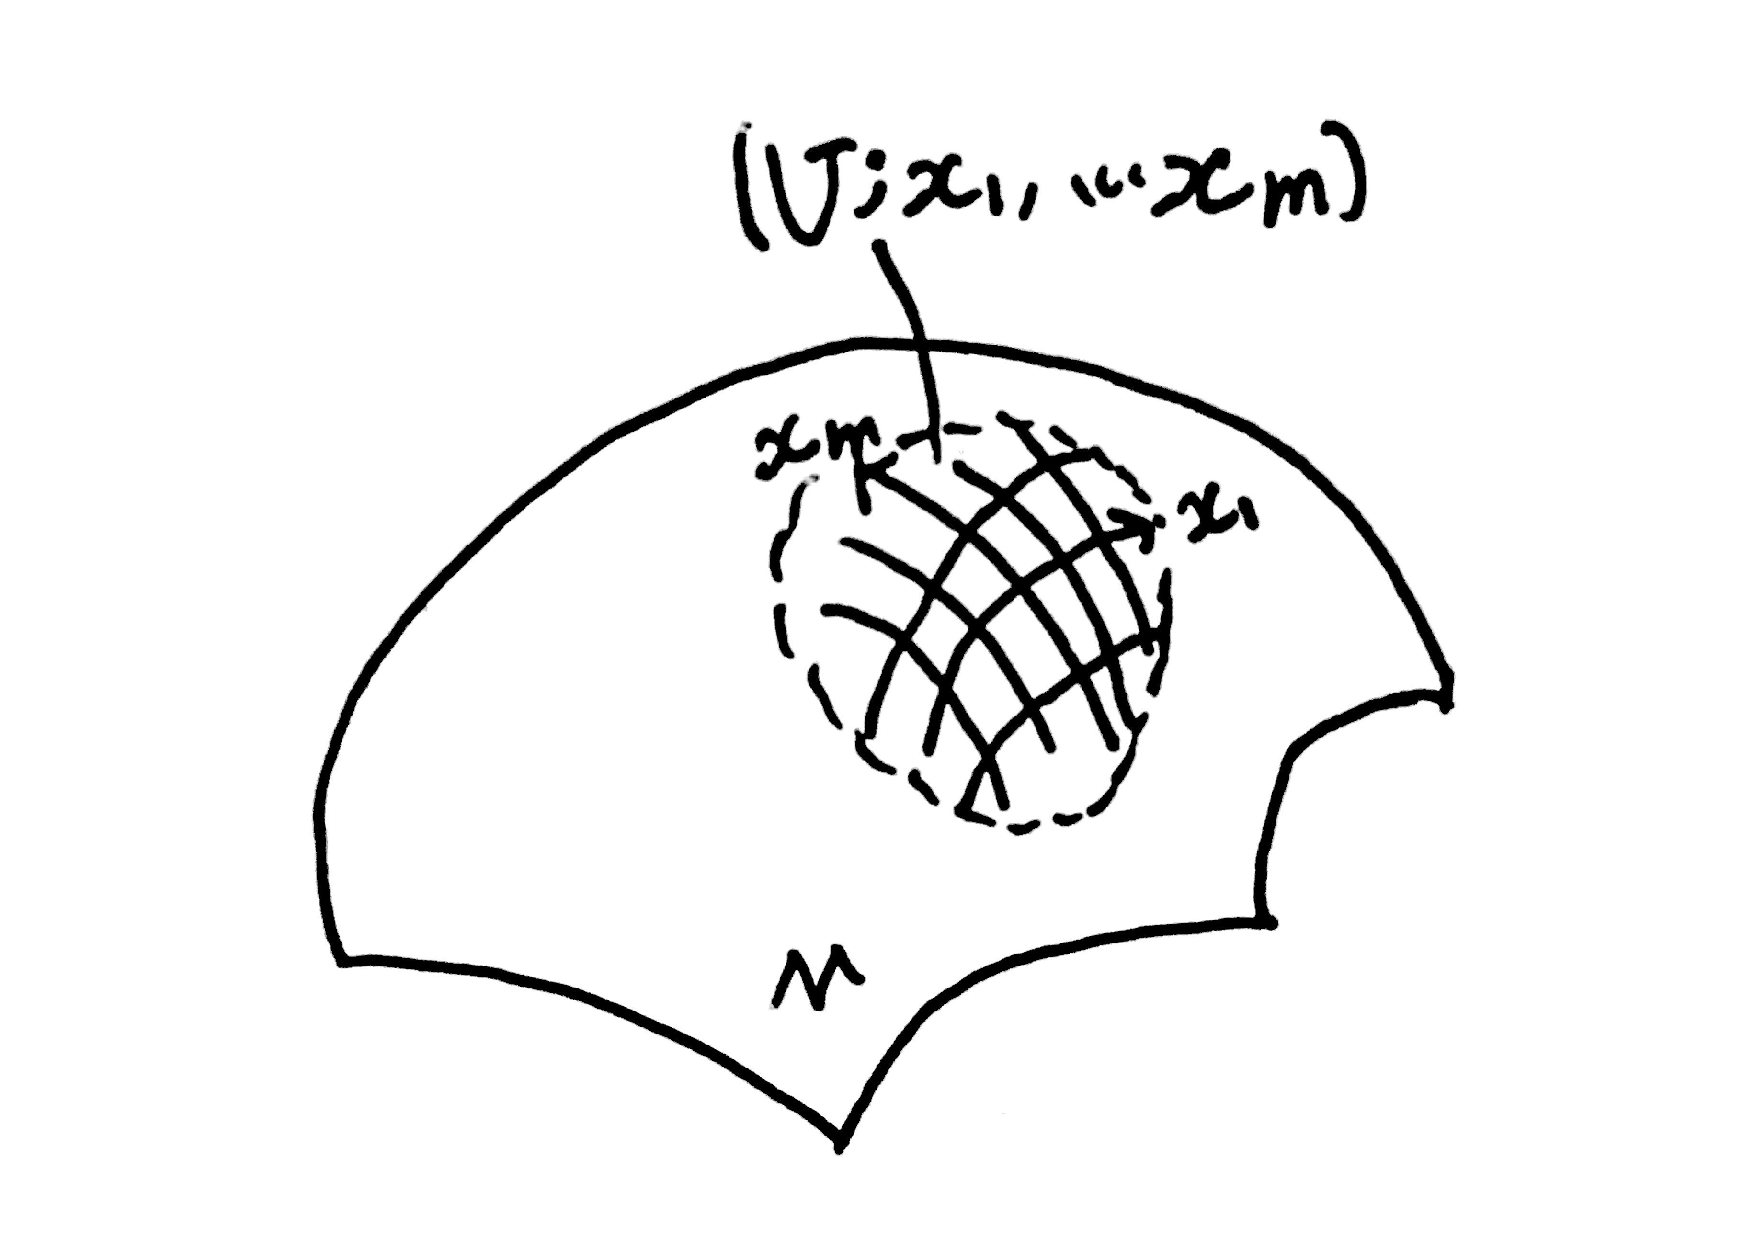
\includegraphics[keepaspectratio, scale=0.2]{DrawnLocalCoSysBig.pdf}
      \caption{描かれた局所座標系}
      \label{}
    \end{minipage}
    %---- 図はここまで ----------------------
  \end{tabular}
\end{figure}
\end{frame}
\begin{frame}
  \frametitle{}
  \begin{dfn}
    $2$つの座標近傍$(U, \varphi)$, 
    $(V, \psi)$が交わっているとき, 同相写像
    $$\psi \circ \varphi^{-1}:\varphi(U\cap V)\rightarrow \psi(U\cap V)$$
    を$(U, \varphi)$から$(V, \psi)$への座標変換という. 
\end{dfn}
局所座標系が描かれているだけでなく, 重なっている場合は
その間の
座標変換$\psi \circ \varphi^{-1}$が微分可能(
座標近傍の張り合わせが滑らか)なものを考る. 
\begin{figure}[H]
    \centering
    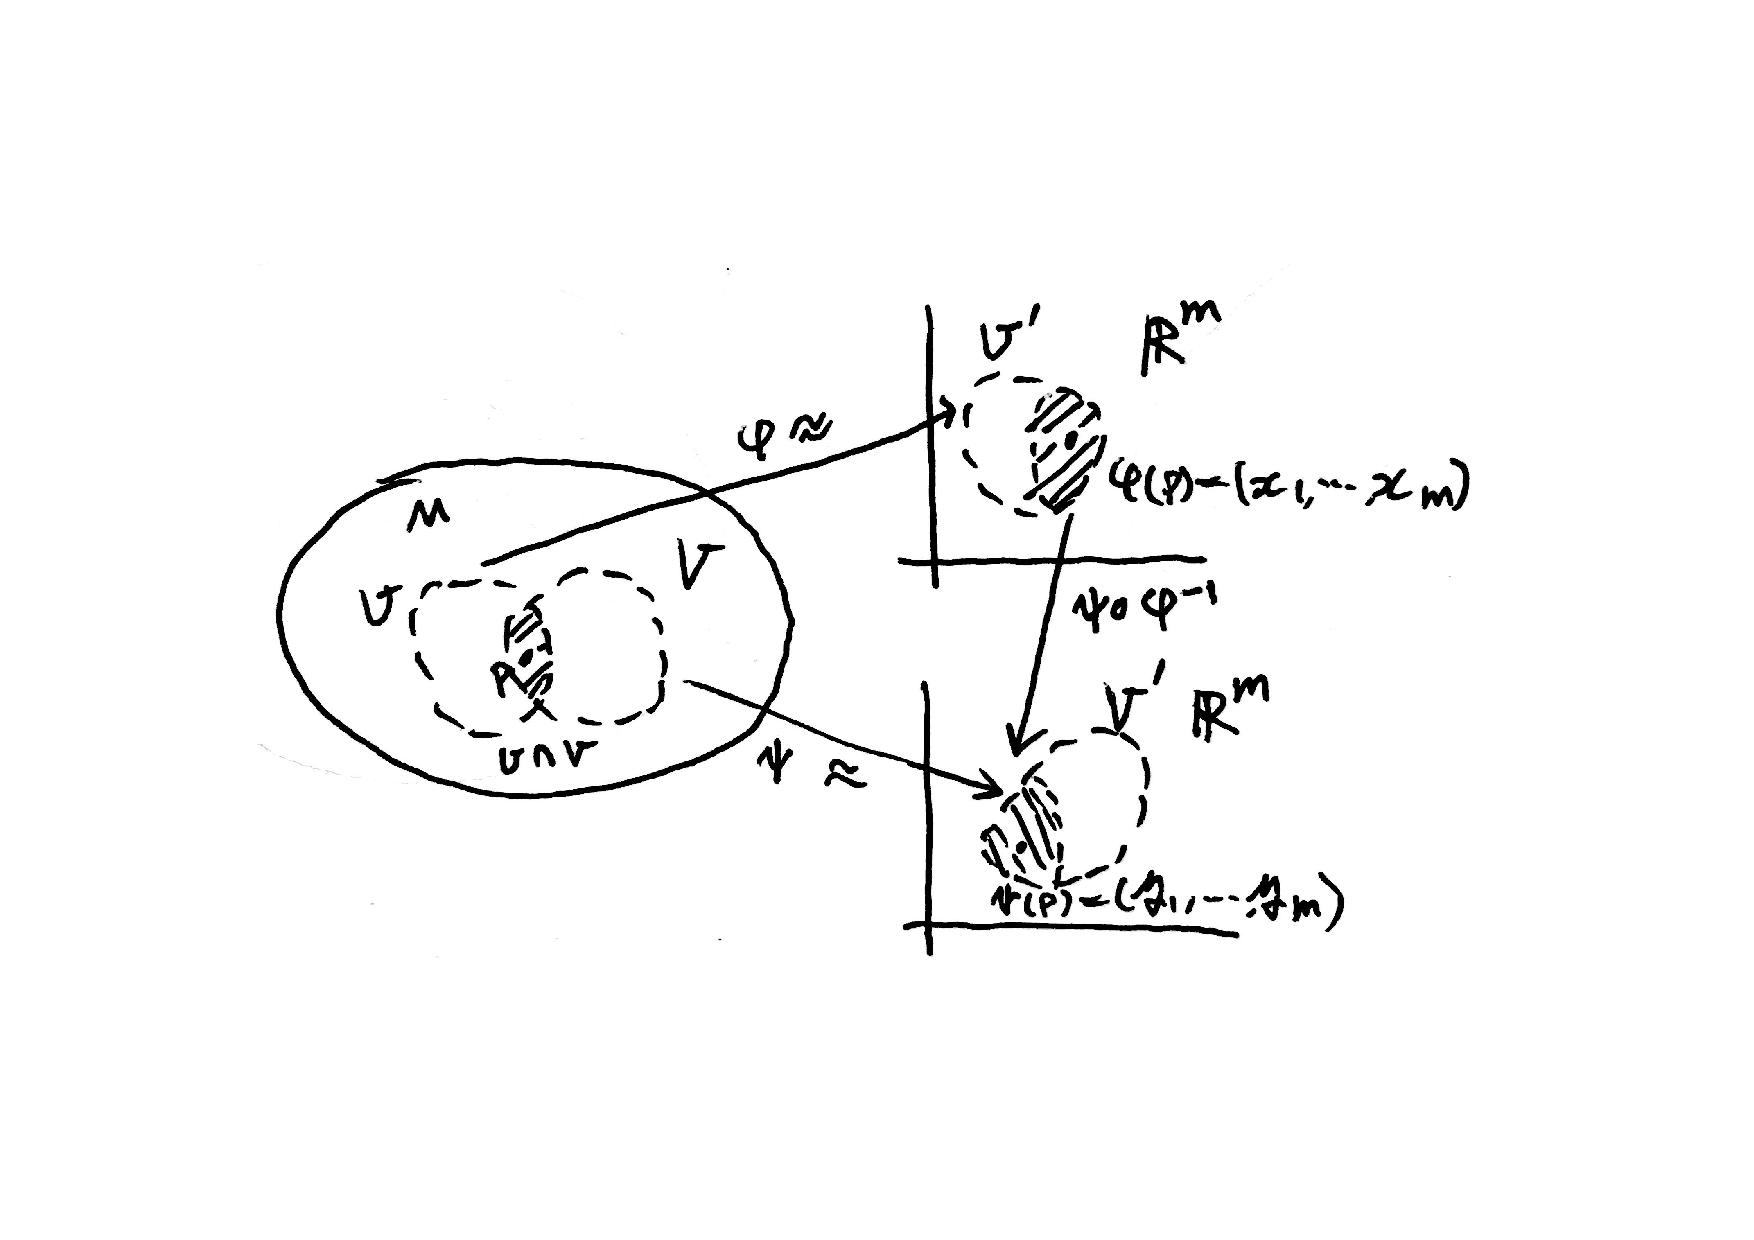
\includegraphics[keepaspectratio, scale=0.3]{coordinateConversionBig.pdf}
    \caption{座標変換$\psi \circ \varphi^{-1}$}
    \label{coordinateConversion}
   \end{figure}
\end{frame}

\begin{frame}
  \frametitle{} 
  \begin{dfn}
  $r$を自然数または$\infty$とする. 位相空間$M$が条件(1), (2), (3)をみたすとき, 
  $M$を$m$次元$\mathit{C}^r$級多様体という. \\
  (1)$M$はハウスドルフ空間である. \\
  (2)$M$は$m$次元座標近傍によって被覆される. \\
  (3)$U_\alpha \cap U_\beta \neq \phi$であるような座標近傍$(U_\alpha, \varphi_\alpha)$, 
  $(U_\beta, \varphi_\beta)$について座標変換
  $$\varphi_\beta \circ \varphi_\alpha^{-1}: \varphi_\alpha(U_\alpha \cap U_\beta)
  \rightarrow \varphi_\beta(U_\alpha \cap U_\beta)$$
  は$\mathit{C}^r$級写像である. 
  \end{dfn}
  \end{frame}
  
  \section{多様体の例}
  \begin{frame}
  \frametitle{多様体の例}
  \begin{thm}
    $m$次元球面$S^m \in \mathbb{R}^{m+1}$を
    $$S^m=\{(x_1,\cdots x_{m+1})|x_1^2+\cdots +x_{m+1}^2=1\}$$
    と定義すると, $S^m$は$m$次元$C^{\infty}$級多様体である. 
  \end{thm}
  \ \\
  \ \\
  \ \\
    \begin{tikzpicture}[scale=1]
      % 球面の描画
      \draw (0, 0, 0) circle (1);
        % 下半分の楕円の描画
      \draw[dashed] (0, 0) ellipse (1 and 0.3);
  % 2点の座標
      \coordinate (A) at (-0.23-0.04, -0.75);
      \coordinate (B) at (-0.02-0.04, 0.8);
     \coordinate (C) at (-1, 0);
      \coordinate (D) at (0.8, 0);
      
      % 曲線の描画
      \draw[line width=1pt,->] (A) to[bend left] (B);
      \draw[line width=1pt,->] (C) to[bend left] (D);
      
  \node at (0.27, 0.5)  {{\fontsize{9pt}{12pt}\selectfont $(U_i^{\pm}, \varphi_i^{\pm})$}};
  \node at (-1, 0.75)  {$S^2$};
  \end{tikzpicture}
\end{frame}


  \begin{frame}
    $\mathbb{R}^{m+1}$はハウスドルフ空間
        であるから, その部分空間として, $S^m$は
        ハウスドルフ空間である. 
        $S^m$の$2(m+1)$個の開集合
        $U_i^+$, $U_i^-$ $(i=1,\cdots ,m+1)$を
        次のように定義する. 
        $$U_i^+ = \{(x_1, \cdots x_i, \cdots ,x_{m+1})\in S^m|x_i>0\}$$
        $$U_i^- = \{(x_1, \cdots x_i, \cdots ,x_{m+1})\in S^m|x_i<0\}$$
        $S^m$はこれら$U_i^+$, $U_i^-$ $(i=1,\cdots ,m+1)$
        で被覆される. 写像$\varphi_i^+:U_i^+ \rightarrow \mathbb{R}^m$, 
        $\varphi_i^-:U_i^- \rightarrow \mathbb{R}^m$を
        それぞれ次のように定義する. 
        $$\varphi_i^+(x_1,\cdots ,x_i,\cdots, x_{m+1})=(x_1,\cdots ,\hat{x_i},\cdots ,x_{m+1})$$
        $$\varphi_i^-(x_1,\cdots ,x_i,\cdots, x_{m+1})=(x_1,\cdots ,\hat{x_i},\cdots ,x_{m+1})$$
        ここで, $\hat{x_i}$は$x_i$を取り去るという意味である. 
      \end{frame}

  \begin{frame}
    \begin{figure}[H]
      \begin{tabular}{cc}
        %---- 最初の図 ---------------------------
        \begin{minipage}[t]{0.45\hsize}
          \centering
          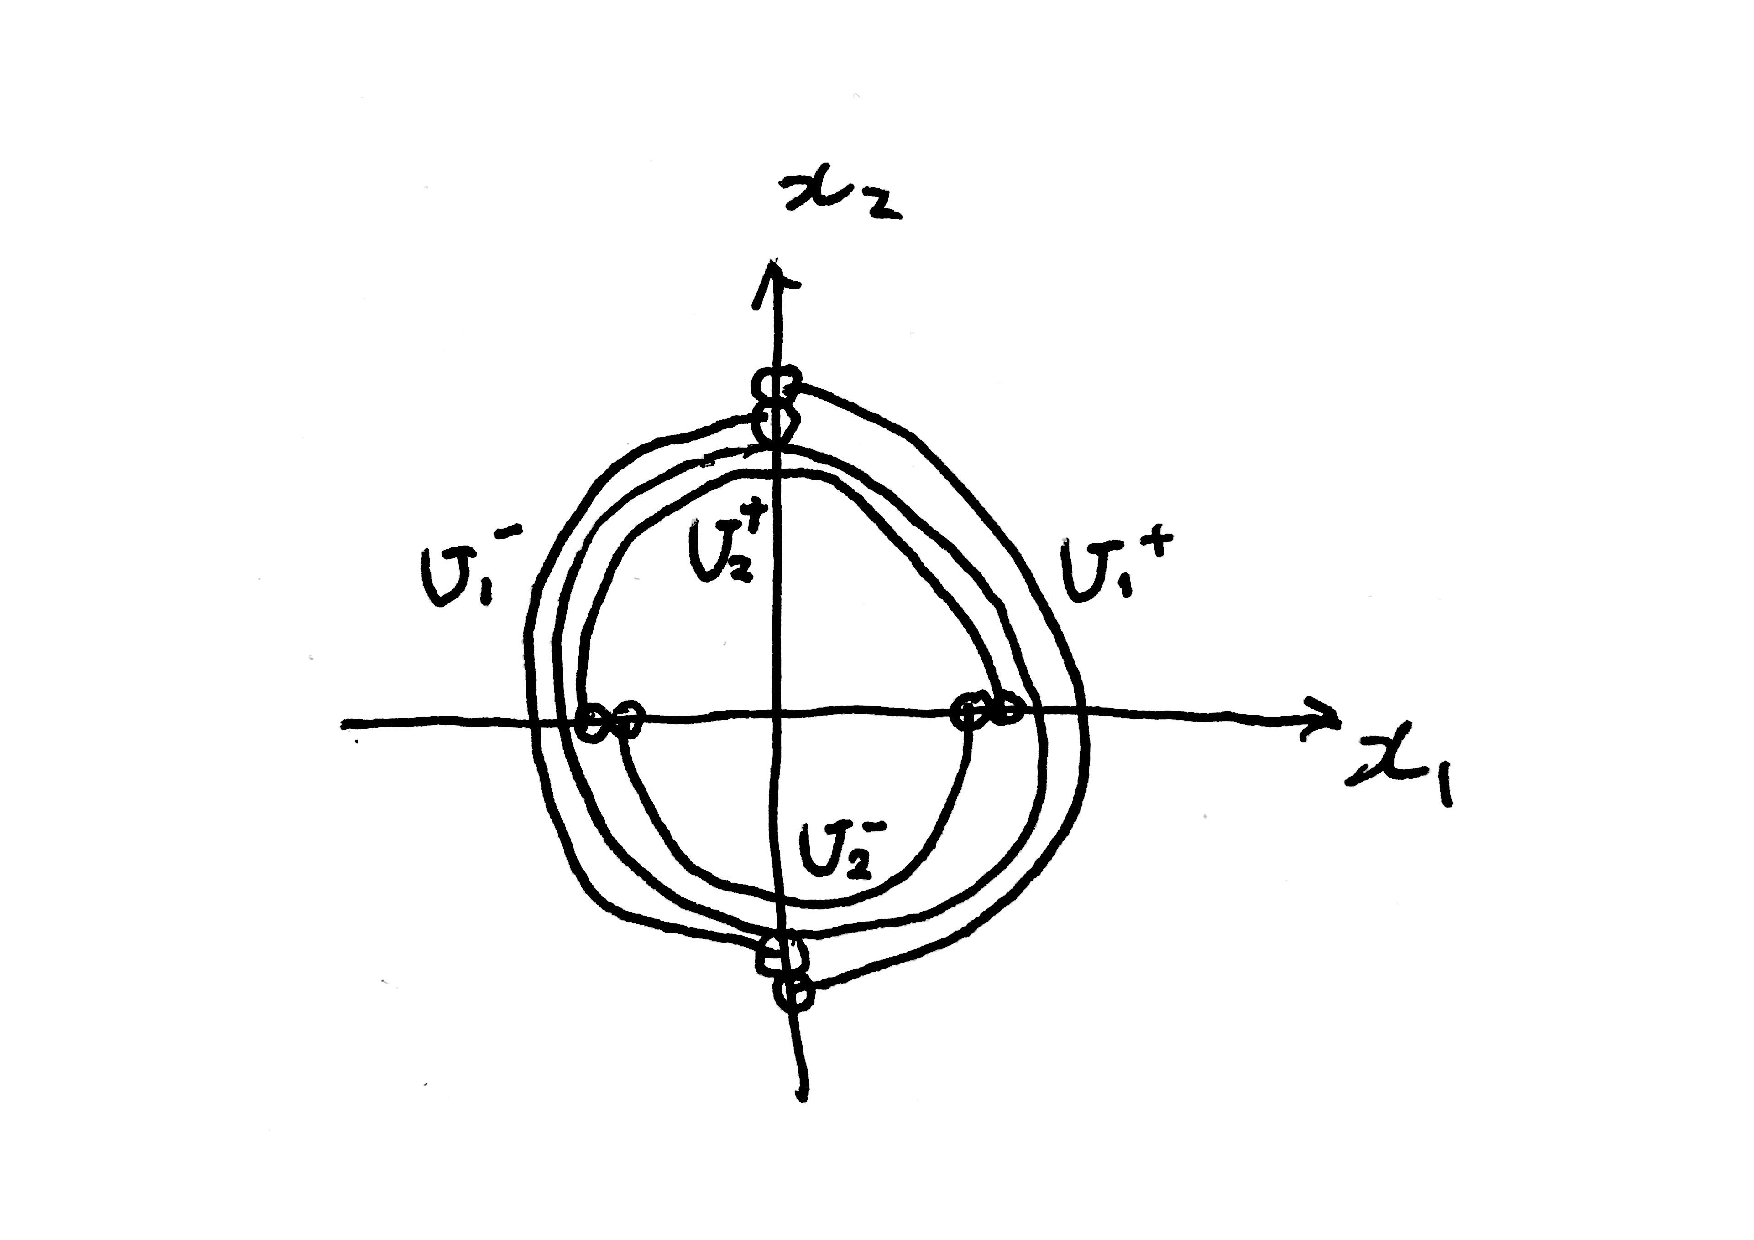
\includegraphics[keepaspectratio, scale=0.25]{localCoSysOfS1_1.pdf}
          \caption{$S^1$の開集合}
          \label{}
        \end{minipage} &
        %---- 2番目の図 --------------------------
        \begin{minipage}[t]{0.45\hsize}
          \centering
          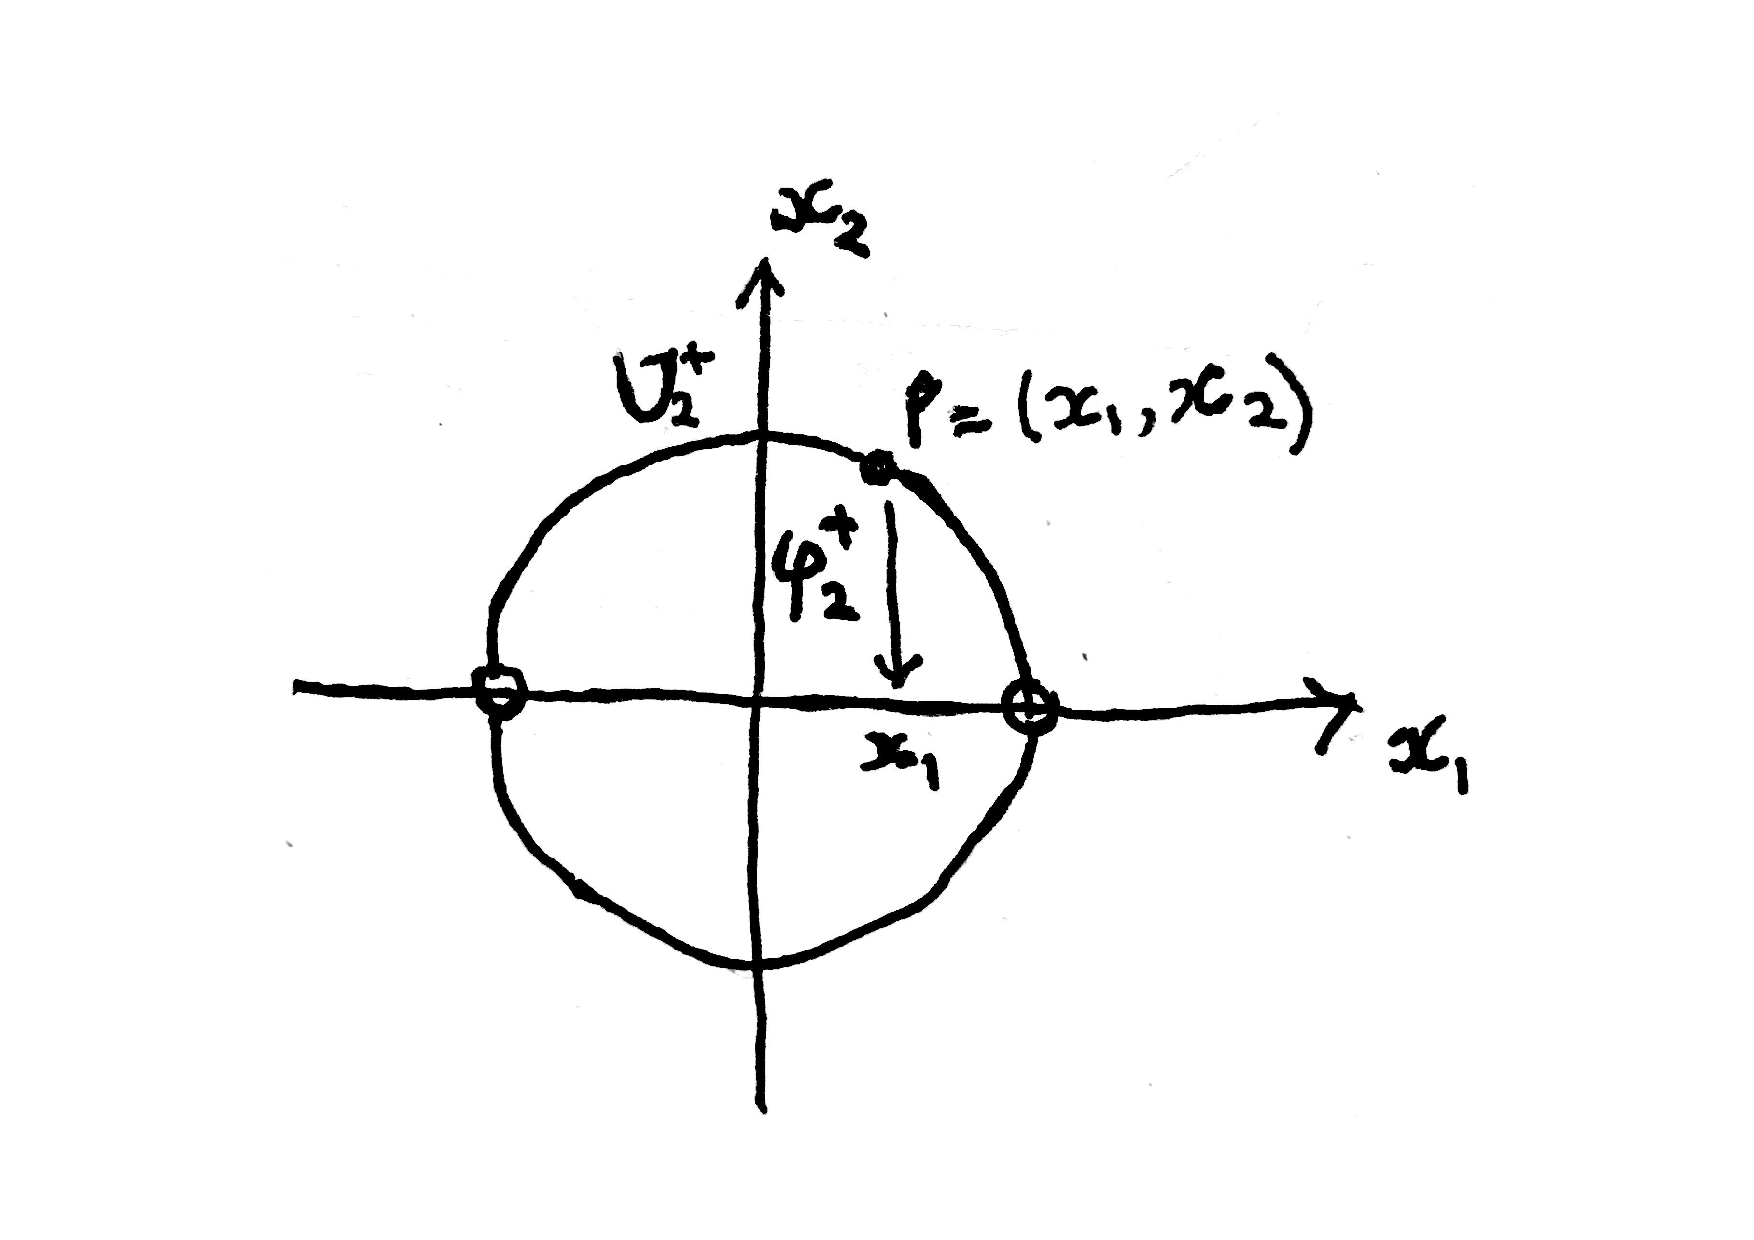
\includegraphics[keepaspectratio, scale=0.25]{localCoSysOfS1_2.pdf}
          \caption{$S^1$の局所座標系}
          \label{}
        \end{minipage}
        %---- 図はここまで ----------------------
      \end{tabular}
    \end{figure}

    このとき, 
    $\varphi_i^+$, $\varphi_i^-$はそれぞれ, $U_i^+$, 
    $U_i^-$から$\mathbb{R}^m$への射影であるから, 同相写像であり, 
    すべての座標変換$\varphi_b^+\circ(\varphi_a^+)^{-1}\ 
    (1\leq a, b\leq 2(m+1))$が$C^{\infty}$級であることが確かめられる. 
    よって, $S^m$は$m$次元$C^{\infty}$級多様体であることがわかる. 
\end{frame}

\section{$C^s$級写像とその微分}
\begin{frame}
    \frametitle{$C^s$級写像とその微分}
  \begin{dfn}\label{def:C^s map}
    $C^r$級多様体$M$($m$次元), $N$
    ($n$次元)間の写像
    $f:M\to N$が$1$点$p\in M$において
    $C^s$級であるとは, $p$を含む$M$の$C^r$級
    座標近傍$(U,\varphi)$と
    $f(p)$を含む$N$の
    座標近傍$(V,\psi)$が存在して, 
    \begin{itemize}
        \item[(1)]$f(U)\subset V$
        \item[(2)]$(U,\varphi)$と
        $(V,\psi)$に関する$f$の
        局所座標表示
        $\psi\circ f\circ \varphi^{-1}$
        が$C^s$級である.
        (ただし, $0\leq s \leq r \leq \infty$) 
    \end{itemize}
    この$2$つの条件が成り立つことである. 
    $f$が任意の点$p\in M$で$C^s$級であるとき, 
    $f$は$C^s$級写像であるという. 
  \end{dfn}
  \begin{figure}[H]
    \centering
    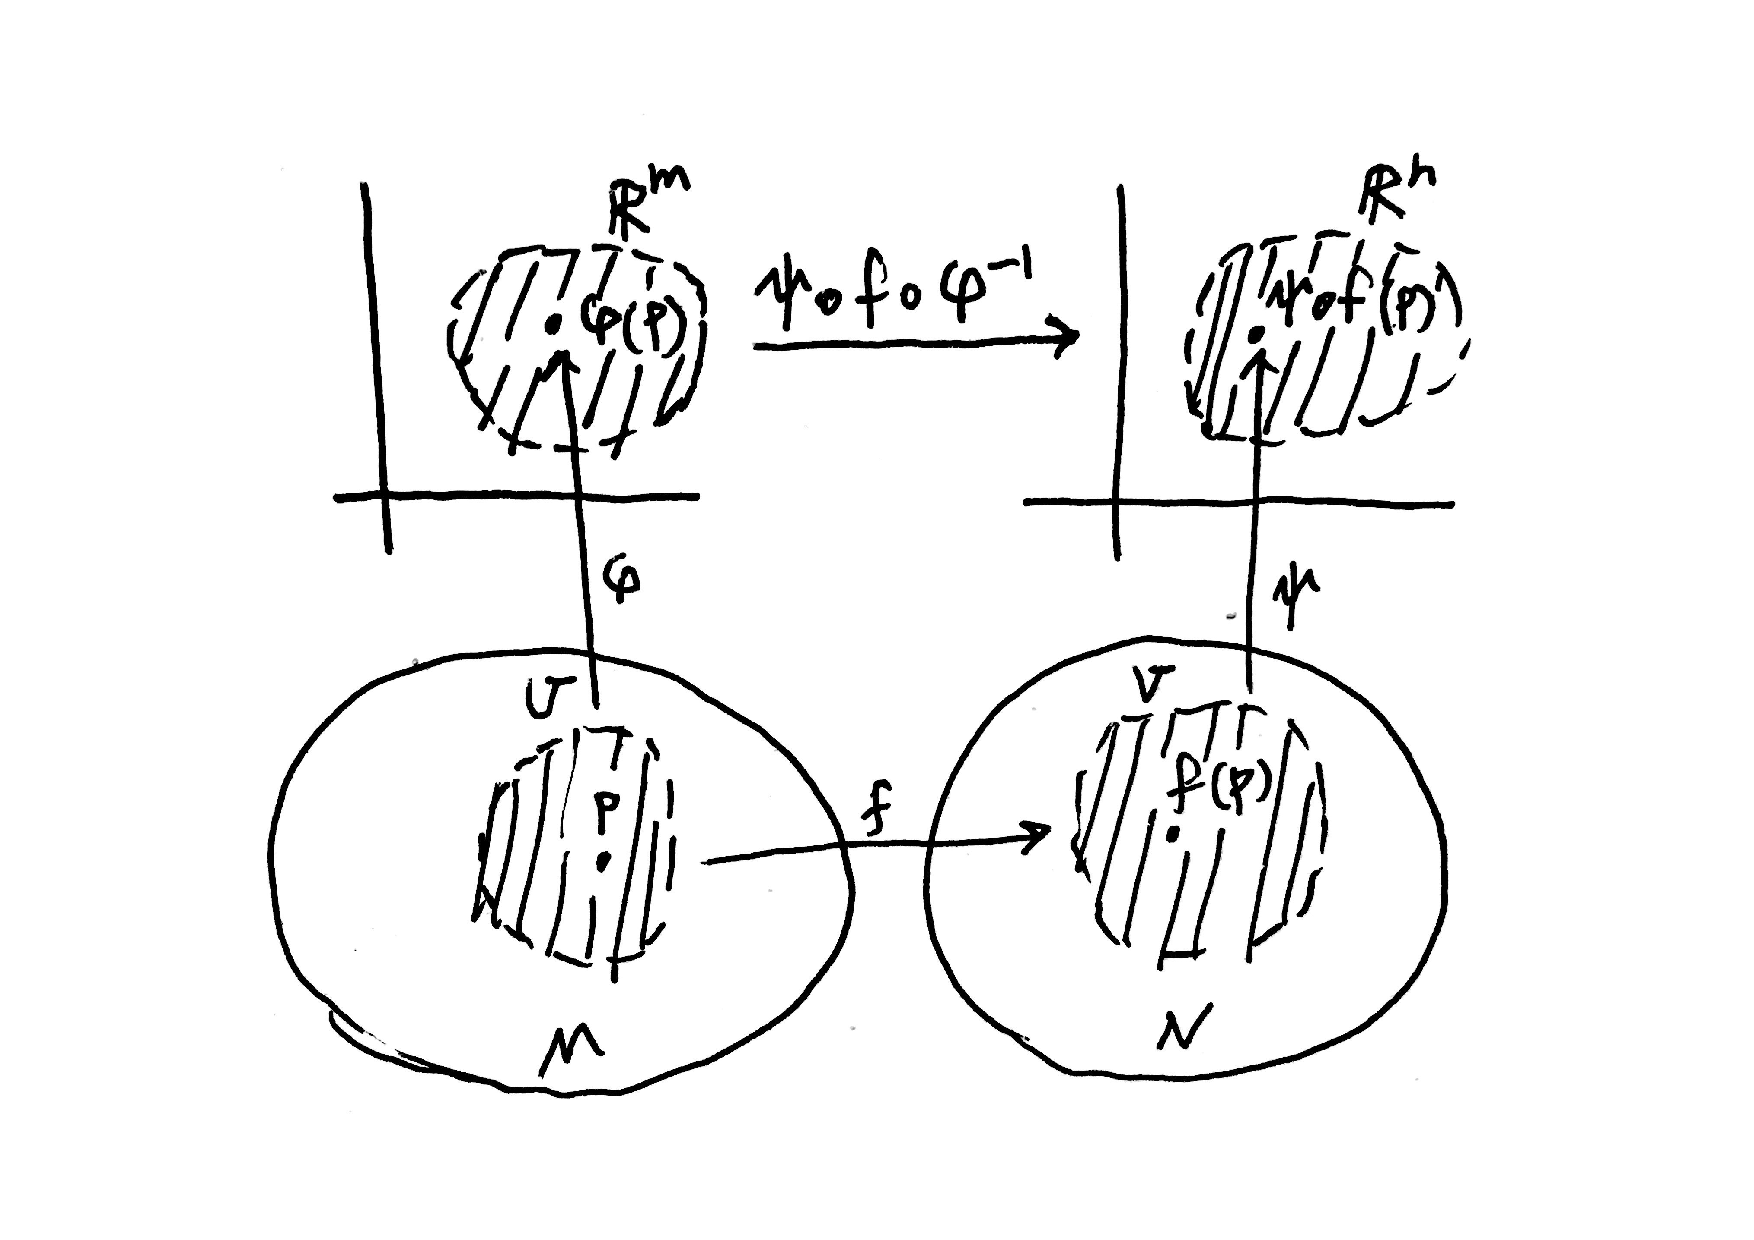
\includegraphics[keepaspectratio, scale=0.15]
         {Csmap.pdf}
    \caption{$f$と$\psi\circ f\circ \varphi^{-1}$
    の関係}
    \label{Csmap}
  \end{figure}
\end{frame}


\begin{frame}
  \frametitle{}
  \begin{dfn}\label{def:C^s deffeomorphism}
    $M$, $N$を$C^r$級多様体とする. $f:M\to N$
    が$C^s$級微分同相写像であるとは, 次の条件
    (1), (2)を満たすことをいう. 
    \begin{itemize}
        \item[(1)]
        $f:M\to N$は全単射($1$対$1$かつ上への写像)
        である. 
        \item[(2)] 
        $f:M\to N$と$f^{-1}:N\to M$はともに$C^s$
        級写像である. 
    \end{itemize}
\end{dfn}
\begin{thm}
  $m$次元$C^r$級多様体, $M$に座標近傍系
  $\mathcal{S}=
   \{(U_\alpha, \varphi_\alpha)\}_{\alpha\in A}$
   が与えられているとする. 
   $V$を$M$の開集合, 
   $V'$を$\mathbb{R}^m$の開集合とし,  
   $\varphi:V\to V'$を$C^r$級微分同相写像
   であるとすると, $\mathcal{S}$に$(V,\psi)$を
   加えた集合
   $\mathcal{S}\cup (V,\psi)$も
   $C^r$級座標近傍系になる. 
   \end{thm}
\end{frame}
\begin{frame}
  \frametitle{}
  \begin{dfn}
  このような$(V,\psi)$の全体集合
  $\mathcal{M}=\mathcal{M}(\mathcal{S})$を
  $\mathcal{S}$から決まる
  $M$の$C^r$級極大座標近傍系という.
  \end{dfn}
  これによって, いくらでも小さい開近傍$U'$や, 
  新しい局所座標系$\varphi '$による座標近傍
  $(U',\varphi ')$も同時に考えら
  れるようになる. 
  \begin{figure}[H]
    \centering
    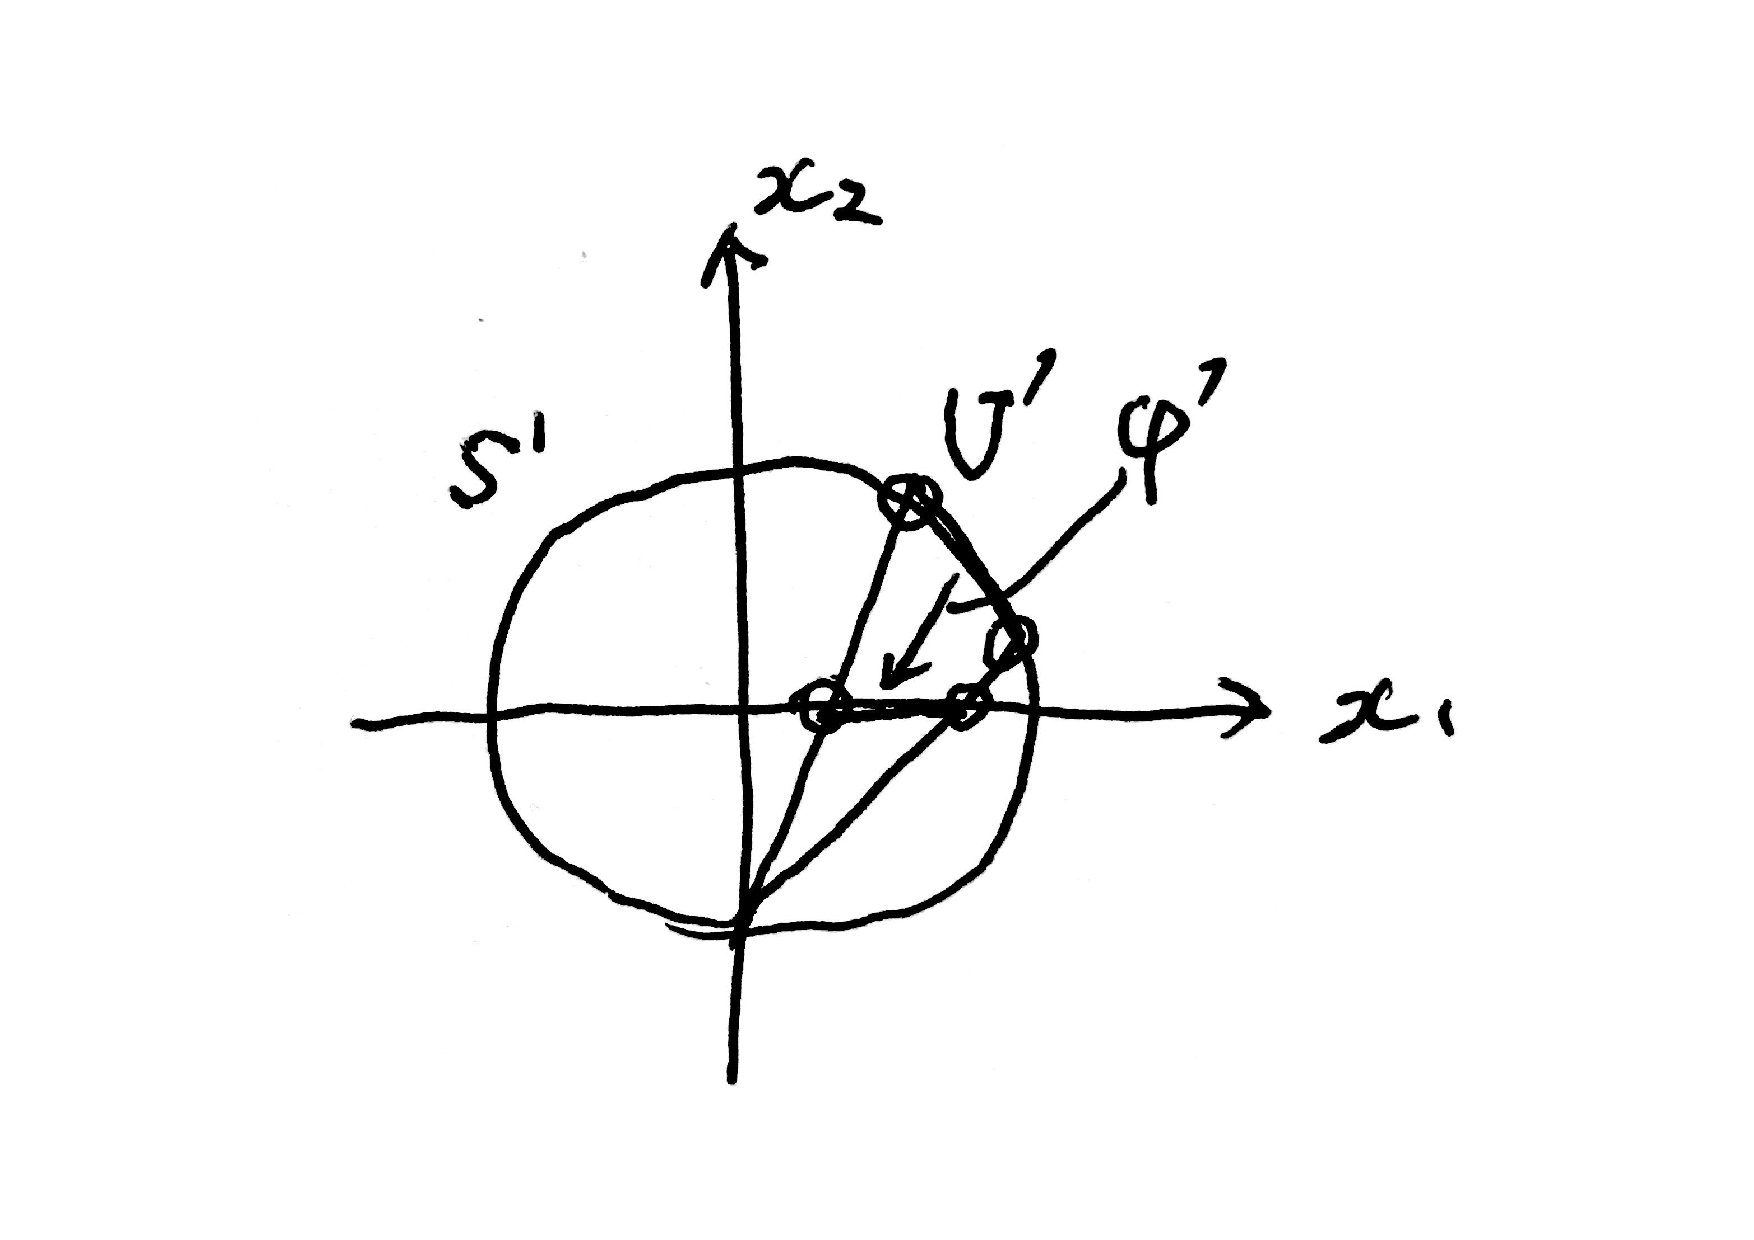
\includegraphics[keepaspectratio, scale=0.25]{stereoprojection.pdf}
    \caption{小さい$U'$とステレオ投影$\varphi '$}
    \label{}
\end{figure}
\end{frame}


\begin{frame}
  \frametitle{}
  \begin{dfn}
    $p\in M$のまわりの座標近傍$(U,\varphi)$上の
    $C^r$級関数$f:M\to \mathbb{R}$に, $p$における$x_i$
    方向の偏微分係数を対応させる操作を
    $$\left(\frac{\partial}{\partial x_i}
    \right)_p:f\mapsto 
    \frac{\partial f\circ \varphi^{-1}}{\partial x_i}(
      \varphi(p))$$
    と表す. 
  \end{dfn}
  和と$a$倍($a\in \mathbb{R}$)を
  $$\left(\frac{\partial}{\partial x_i}
  \right)_p+\left(\frac{\partial}{\partial x_j}
  \right)_p:f\mapsto 
  \frac{\partial f\circ \varphi^{-1}}{\partial x_i}(
    \varphi(p))+\frac{\partial f\circ \varphi^{-1}}{\partial x_j}(
      \varphi(p))$$
  $$\left(\frac{\partial}{\partial x_i}
  \right)_p:f\mapsto 
  a\frac{\partial f\circ \varphi^{-1}}{\partial x_i}(
    \varphi(p))$$
  と定義すると, 
  $\left(\frac{\partial}{\partial x_1}\right)_p, 
  \cdots 
  \left(\frac{\partial}{\partial x_m}\right)_p$
  の$1$次結合全体の集合
  はベクトル空間となり, 
  $m$個のベクトル
  $\left(\frac{\partial}{\partial x_1}\right)_p, 
  \cdots 
  \left(\frac{\partial}{\partial x_m}\right)_p$
  はその基底になっている. 
\end{frame}

\begin{frame}
  \begin{dfn}\label{def:tangent vector space}
    $m$個のベクトル
    $\left(\frac{\partial}{\partial x_1}\right)_p, 
    \cdots 
    \left(\frac{\partial}{\partial x_m}\right)_p$
    の張るベクトル空間を, 点$p$
    における$M$の接ベクトル空間とよび, 
    $T_p(M)$
    という記号で表す. 接ベクトル空間$T_p(M)$の
    元$\boldsymbol{v}\in T_p(M)$を接ベクトルとよぶ. 
  \end{dfn}
  \begin{figure}[H]
        \centering
        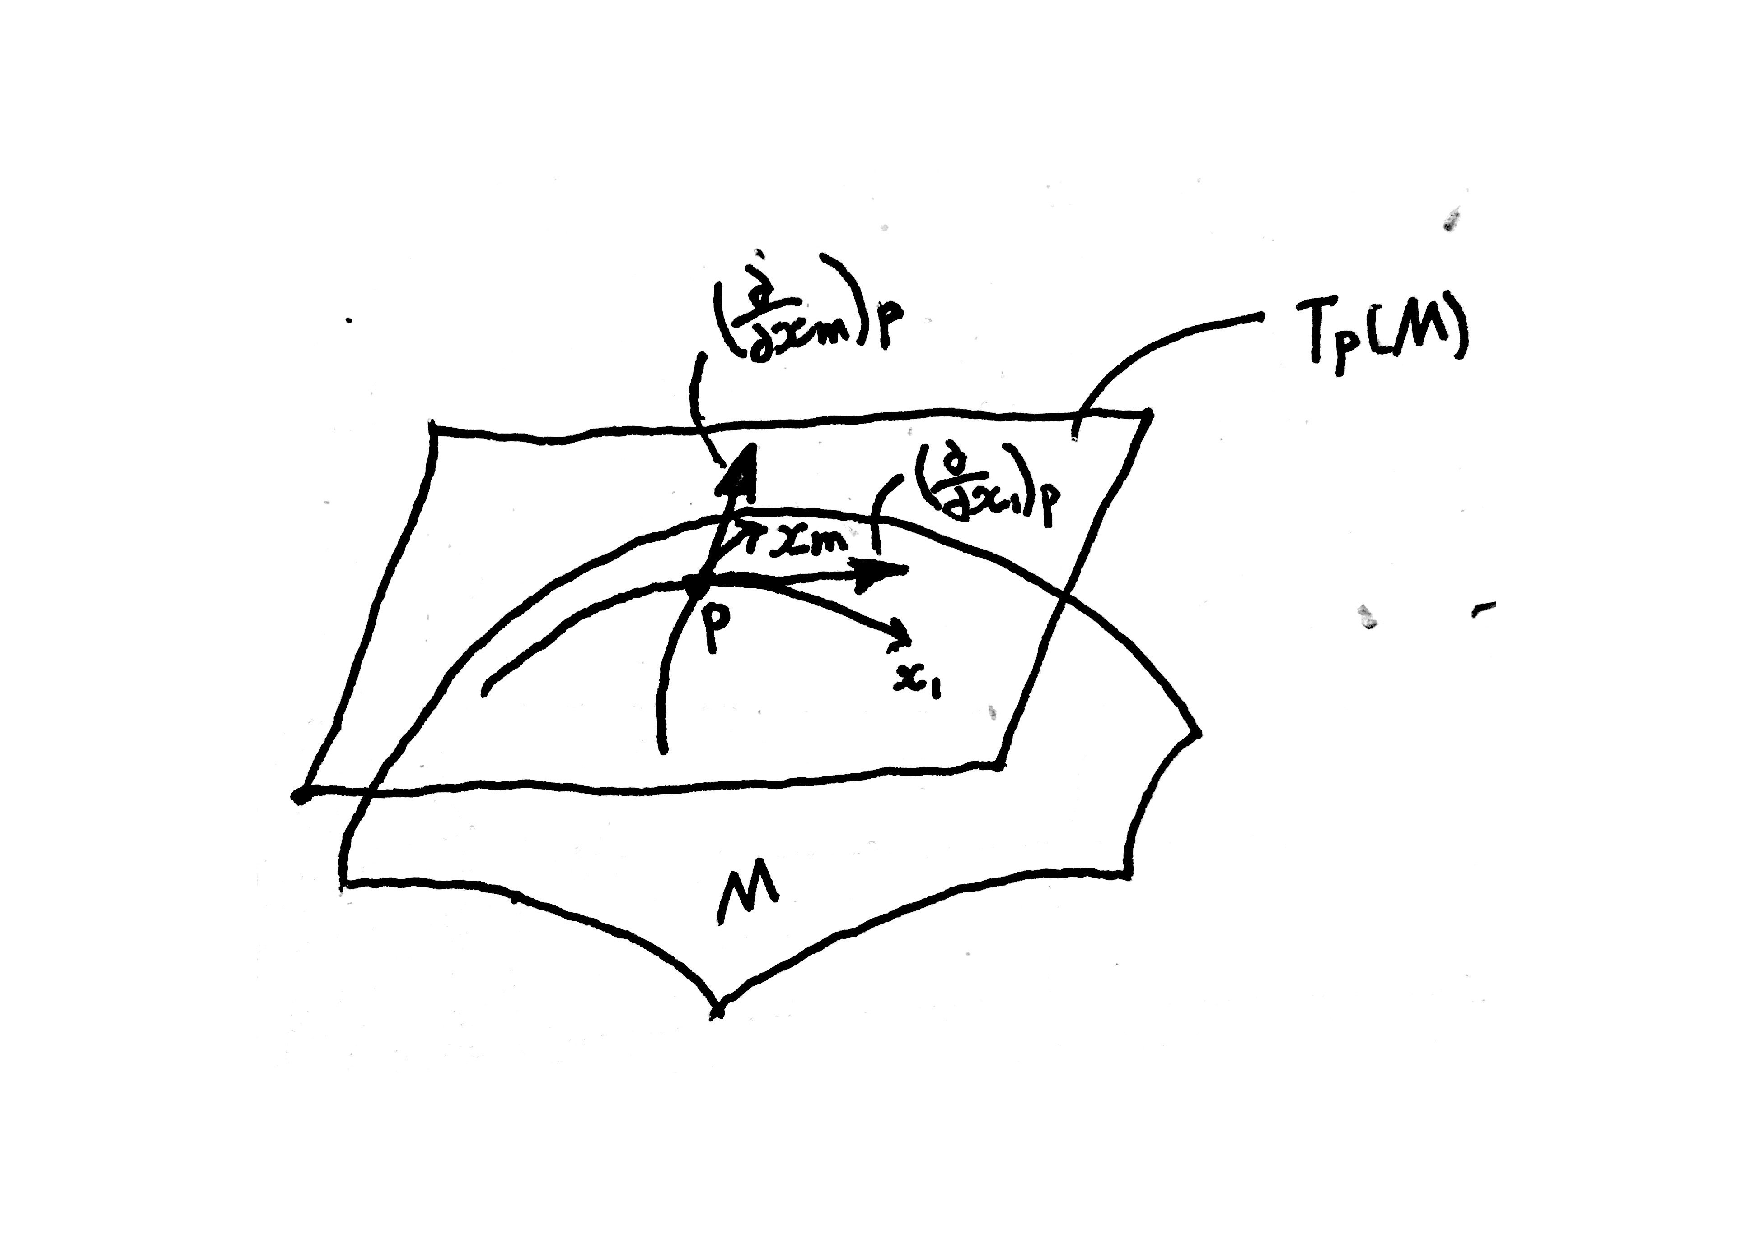
\includegraphics[keepaspectratio, scale=0.28]{tangentVectorSpace_2.pdf}
        \caption{$T_p(M)$のイメージ}
        \label{}
  \end{figure}
\end{frame}

  % \begin{frame}
  %   \frametitle{}
  %   \begin{prop}
  %     $T_p(M)$は点$p$のまわりの局所座標系のとり方に
  %     よらず一意に定まる. つまり, 点$p$のまわりで
  %     $(x_1,\cdots ,x_m)$と別の局所座標系
  %     $(y_1,\cdots ,y_m)$を選んだとき, 
  %     方向微分
  %     $$\left(\frac{\partial}{\partial y_1}\right)_p, 
  %     \cdots ,
  %     \left(\frac{\partial}{\partial y_m}\right)_p$$
  %     の張る$D_p^r(M)$の部分ベクトル空間は, 
  %     $$\left(\frac{\partial}{\partial x_1}\right)_p, 
  %     \cdots ,
  %     \left(\frac{\partial}{\partial x_m}\right)_p$$
  %     の張る部分ベクトル空間に一致する. 
  % \end{prop}
  % \end{frame}

\begin{frame}
  \frametitle{}
  \begin{dfn}\label{def:differential}
    任意の接ベクトル$\boldsymbol{v}\in T_p(M)$
    を$\boldsymbol{v}=
    \sum_{i=1}^{m}v_i\left(\frac{\partial}
    {\partial x_i}\right)_p$とし, $m$次元
    数ベクトル$(v_1,\cdots ,v_m)$とみなすとき, 
     $$(df)_p:T_p(M)\to T_{f(p)}(N),\ 
    \begin{pmatrix}
      v_1\\
      \vdots \\
      v_m
    \end{pmatrix}
    \mapsto
    (Jf)_p
    \begin{pmatrix}
      v_1\\
      \vdots \\
      v_m
    \end{pmatrix}$$
    を, 点$p$における$f:M\to N$
    の微分とよぶ. ただし, $(Jf)_p$は
    点$p$におけるヤコビ行列
    $$(Jf)_p=
    \left(
    \begin{array}{ccc}
      \frac{\partial (\psi\circ f\circ \varphi^{-1})_1}{\partial x_1}(\varphi(p))&\cdots &\frac{\partial (\psi\circ f\circ \varphi^{-1})_1}{\partial x_m}(\varphi(p))\\
      \vdots &\ddots& \vdots \\
      \frac{\partial (\psi\circ f\circ \varphi^{-1})_n}{\partial x_1}(\varphi(p))&\cdots &\frac{\partial (\psi\circ f\circ \varphi^{-1})_n}{\partial x_m}(\varphi(p)) 
    \end{array} 
    \right)$$
    であるとする. 
  \end{dfn}
\end{frame}

\section{写像の局所的性質}
\begin{frame}
  \frametitle{写像の局所的性質}
  \begin{thm}\label{theo:f^(-1)theorem}
    $(df)_p:T_p(M)\to T_f(p)(N)$が線型写像として
    同型(det$(Jf)_p\neq 0$)なら, $f$は$p$のある開近傍から$f(p)$の
    ある開近傍への$C^r$級微分同相写像である. 
    すなわち, $p$の開近傍$U$と$f(p)$の開近傍$V$
    が存在して, $f(U)=V$となり, かつ, 
    $f|U:U \to V$は$C^r$級微分同相写像である. 
  \end{thm}
  これを逆関数の定理という. 
  \begin{ex}
    $f:\mathbb{R}\to \mathbb{R}, f(x)=x^2$と
    すると, $(Jf)_x=2x$となり, $x\neq 0$のとき
    det$(Jf)_x\neq 0$となるので, 十分
    小さい$p$の開近傍上$U$で$f|U$
    は$C^\infty$級微分同相写像である. 
    実際$p>0$のとき, $p$の十分小さい開近傍
    $U$で$f|U^{-1}:
    f|U^{-1}(x)=\sqrt{x}$が
    存在し, $C^\infty$
    級であるので, $f|U$が
    $C^\infty$級微分同相写像であることがわかる.
  \end{ex}
\end{frame}

\begin{frame}
  \frametitle{}
  \begin{thm}\label{theo: projection theorem}
    $f:M\to N$を$C^r$級写像とする. ある点$p\in M$
    における微分$(df)_p:T_p(M)\to T_f(p)(N)$が上への
    線型写像(rank$(Jf)_p=n$)なら, 点$p$付近での$f$の様子は,
    射影と同じ, つまり, $f(p)$のまわりの局所座標系
    $(y_1, \cdots ,y_n)$に対して
    $p$のまわりの局所座標系
    $(x_1,\cdots ,x_m)$をうまく選んで, $f$
    の局所座標表示
    $(y_1, \cdots ,y_n)=f(x_1,\cdots,x_m)$が
    \begin{eqnarray*}
        y_1&=&f_1(x_1,\cdots ,x_m)=x_{m-n+1}\\
        &\vdots& \\
        y_n&=&f_n(x_1,\cdots ,x_m)=x_m
    \end{eqnarray*}
    であるようにできる. 
  \end{thm}
  これを射影の定理とよぶこととする. 
\end{frame}

\begin{frame}
  $p$のまわりの座標近傍が$(U;x_1, \cdots ,x_m)$
  のとき, 
  $$\varphi(x_1,\cdots ,x_m)=
  (x_1,\cdots ,x_{m-n+1},f_1(x_1\cdots ,x_m),\cdots
  ,f_n(x_1,\cdots ,x_m))$$
  ととるとdet$(J\varphi)_p\neq 0$となり, 逆関数の定理
  を利用して$\varphi|U$が$C^r$級微分同相写像であることがわかる. 
  $(U,\varphi|U)$が新しい$C^r$級座標近傍になり, 
  $p$のまわりの局所座標系$(x_1,\cdots ,x_m)$は
  このように選べば良いことが分かる.
  \frametitle{}
  \begin{figure}[H]
    \centering
    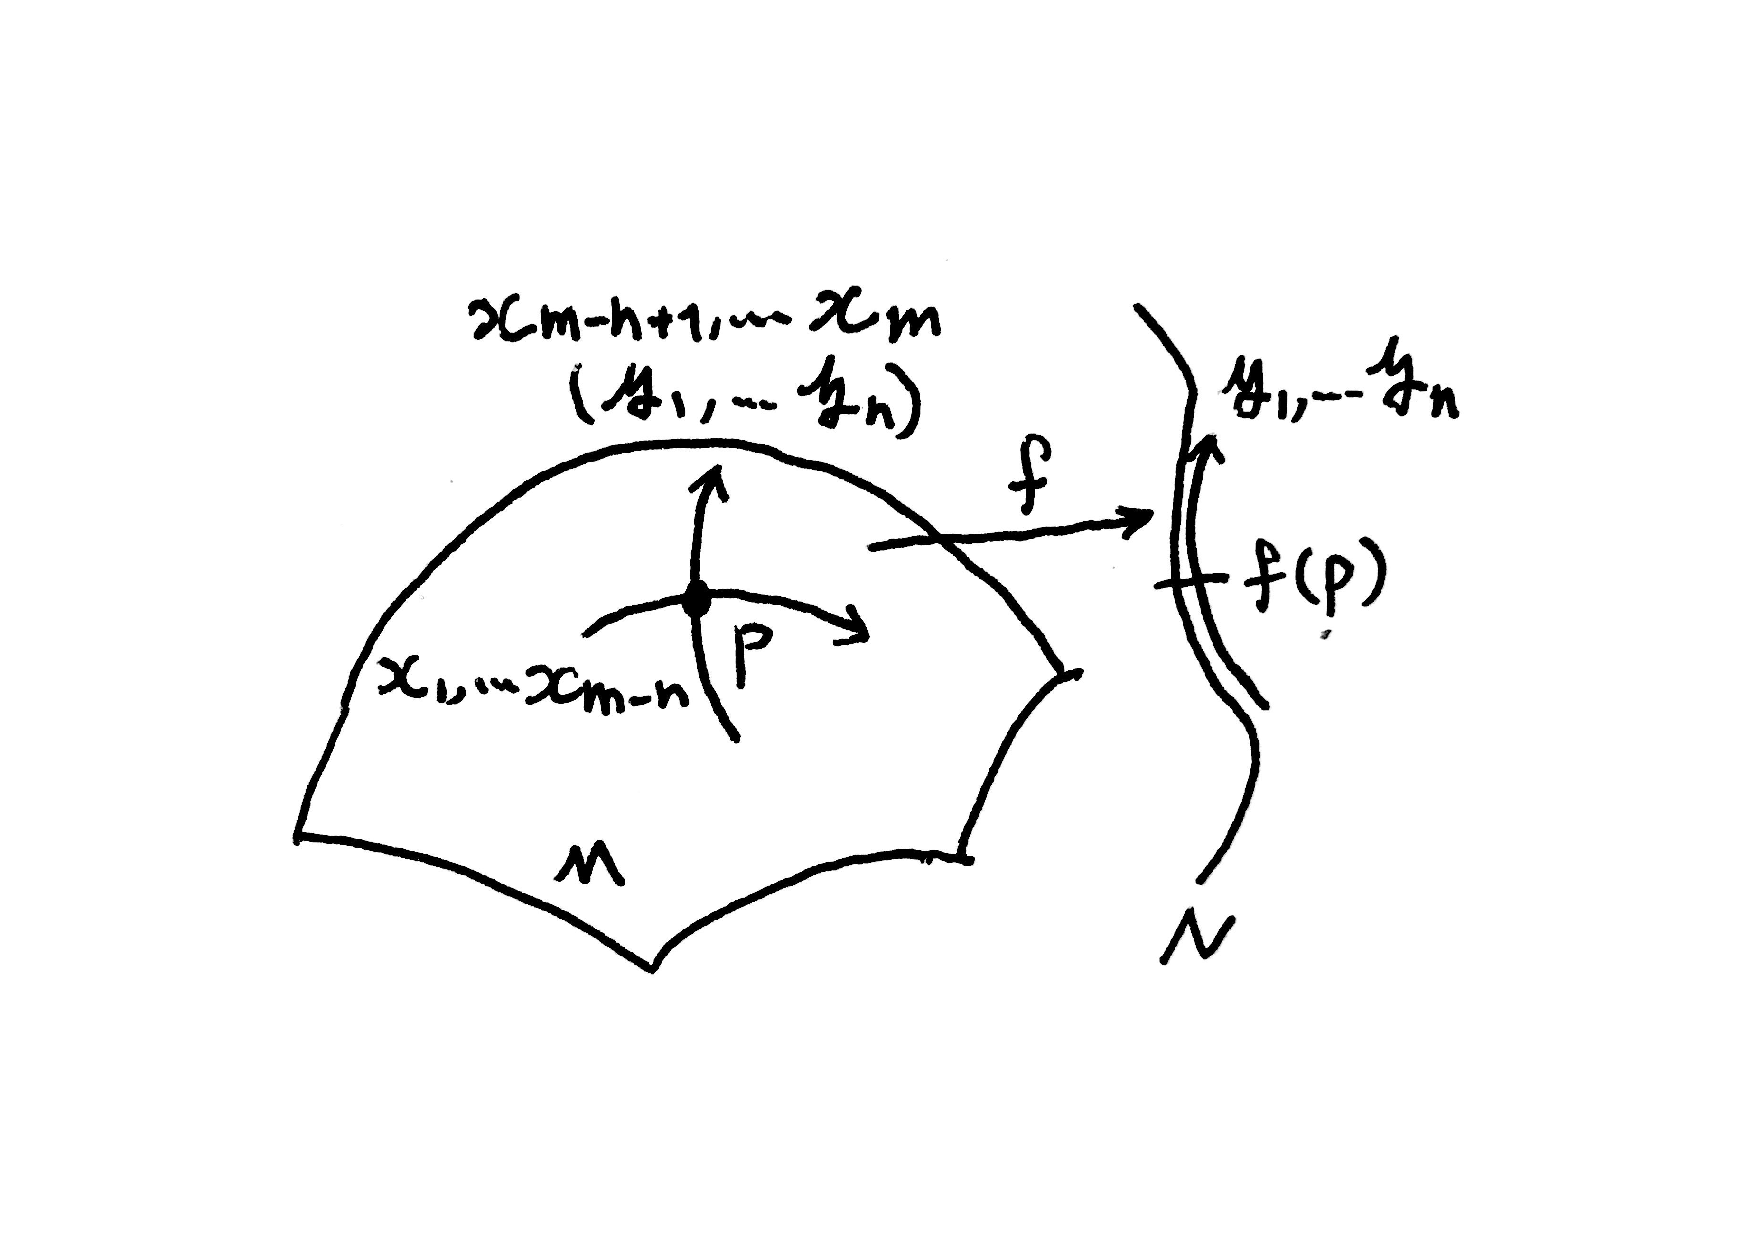
\includegraphics[keepaspectratio, scale=0.35]{projection_new.pdf}
    \caption{射影の様子}
    \label{projectionTheorem}
   \end{figure}
\end{frame}

\begin{frame}
  \frametitle{}
  \begin{dfn}\label{def:C^r-submanifold}
    $n$次元$C^r$級多様体$N$の部分集合$L$が
    $N$の$l$次元$C^r$級部分多様体であるとは, 
    \begin{itemize}
        \item[(1)]$l=n$のとき:$L$が$N$の開集合
        であることである. 
        \item[(2)] $0\leq l<n$のとき:$L$の任意の点$p$
        に対し, $p$を含む$N$の座標近傍$(U;x_1,\cdots ,x_n)$
        が存在して, 
        $$L\cap N=\{(x_1,\cdots ,x_n)\in U|
        x_{l+1}=\cdots =x_n=0\}$$
        が成り立つことである. 
    \end{itemize}
  \end{dfn}
  \begin{figure}[H]
    \centering
    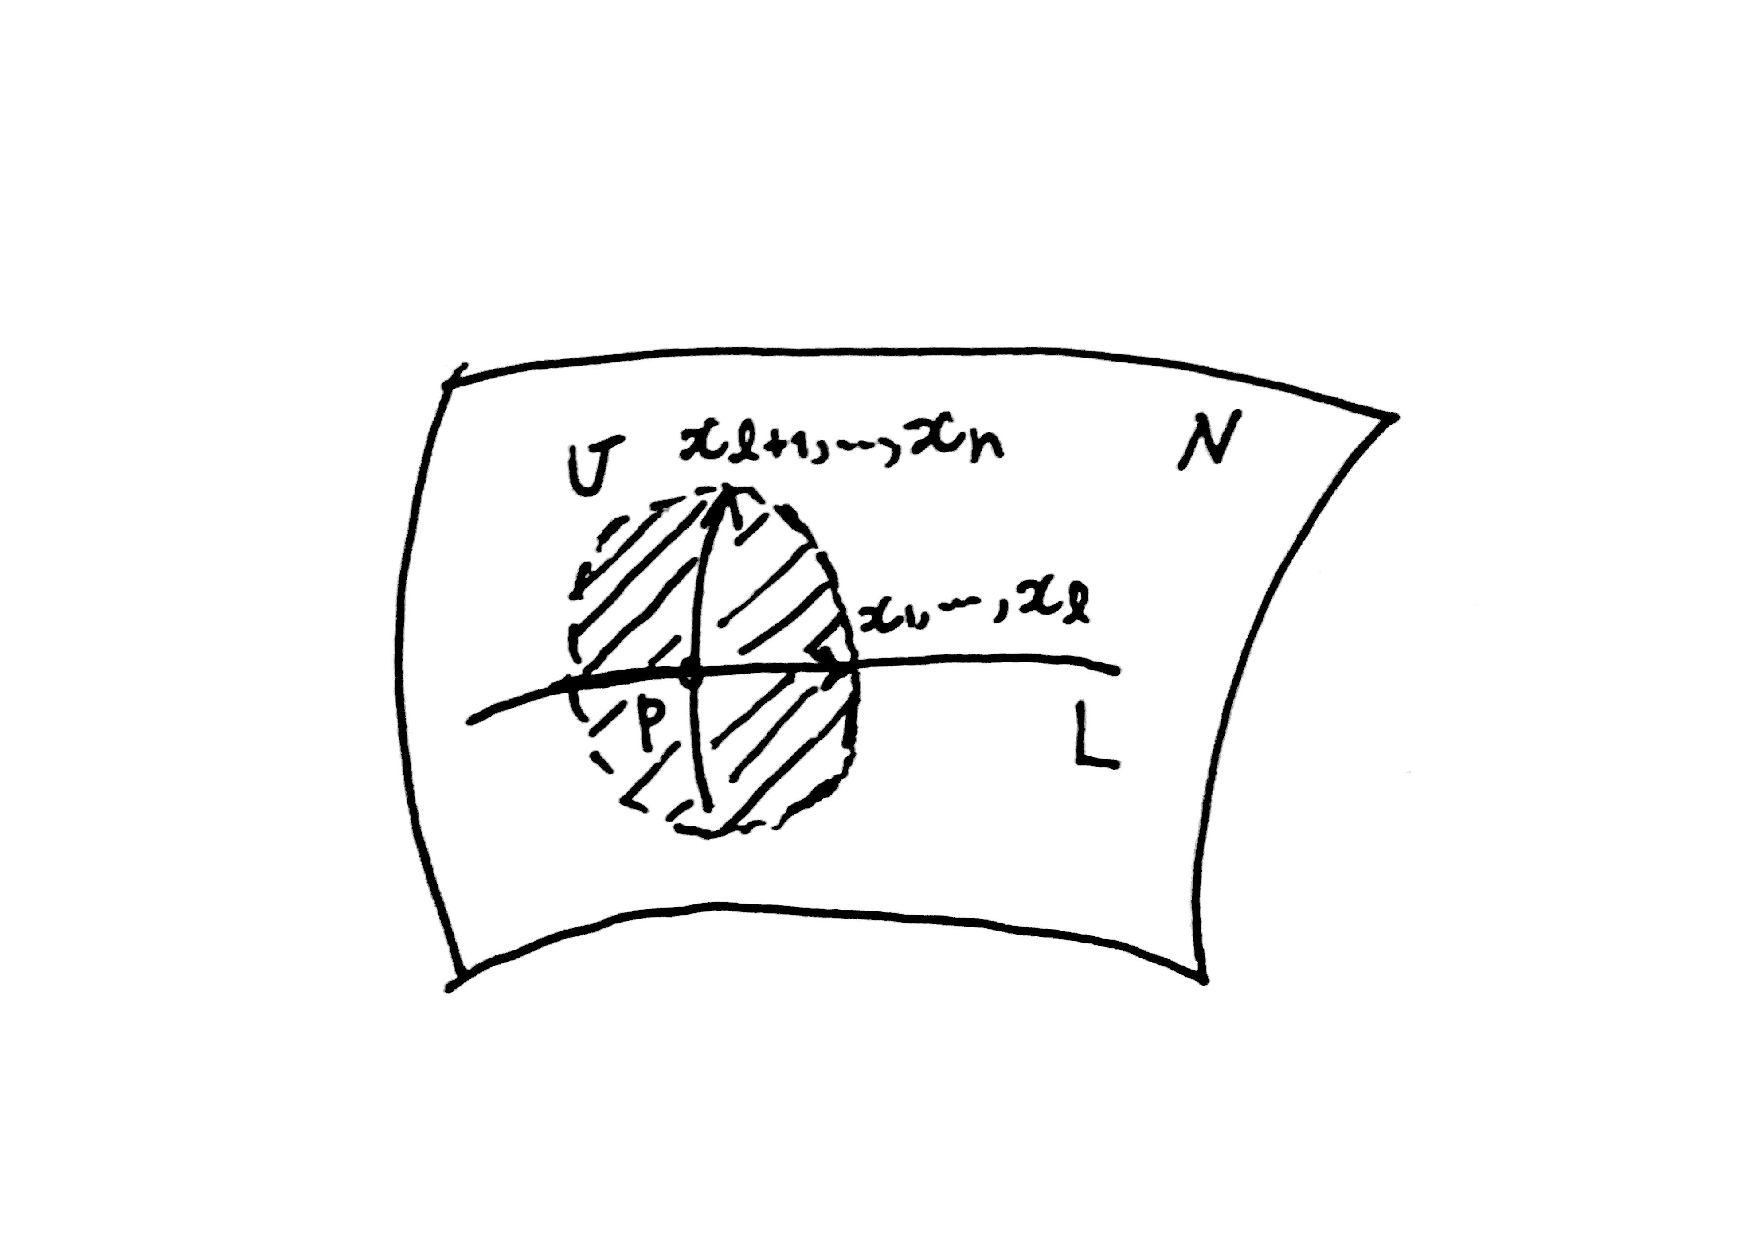
\includegraphics[keepaspectratio, scale=0.2]{CrSubmanifold.pdf}
    \caption{$N$の部分多様体$L$}
    \label{CrSubmanifold}
   \end{figure}
\end{frame}

\begin{frame}
  \frametitle{}
  \begin{prop}\label{prop:dim of C^r-submanifold}
    $n$次元$C^r$級多様体$N$の$l$次元$C^r$級
    部分多様体$L$は, それ自身$l$次元$C^r$級
    多様体である. 
  \end{prop}
\end{frame}
     
\begin{frame}
  \frametitle{}
  \begin{thm}\label{theo:f^{-1}(q) C^r manifold}
    $M$, $N$を$m$次元, $n$次元の$C^r$級多様体, 
    $f:M\to N$を$C^r$級写像とする. $N$のある点
    $q$について, $f(p)=q$となる$M$の各点$p$
    が常にrank$(Jf)_p=n$を満たすとき, 逆像
    $f^{-1}(q)$は$(m-n)$次元$C^r$級多様体
    である. 
  \end{thm}
  $q\in N$の逆像$f^{-1}(q)$に属する任意の点
  $p$に対し, $p$のまわりの座標近傍
  $(U;x_1,\cdots .x_m)$が存在して, 
  $$f^{-1}(q)\cap U
  =\{(x_1,\cdots x_m)\in U|
  x_{m-n+1}=\cdots =x_m=0\}$$
  が成り立つこと
  ($(m-n)$次元$C^r$級
  部分多様体の条件)を証明すればよい. 
\end{frame}

\begin{frame}
  \frametitle{}
    今, $f(p)=q$を満たす$p\in M$について, 常に
    rank$(Jf)_p=n$であるから, $(df)_p$は上への
    写像である. よって, 
    $q$($=f(p)$)のまわりの座標近傍$(V;y_1,\cdots ,y_n)$
    に対して, $(V;y_1,\cdots ,y_n)$は
    点$q$で$y_1=\cdots =y_n=0$となるように
    とっておくと, 射影の定理より
    $p$のまわりの座標近傍$(U;x_1,\cdots ,x_m)$を
    とってきて以下のようにできる. 
    \begin{figure}[H]
      \centering
      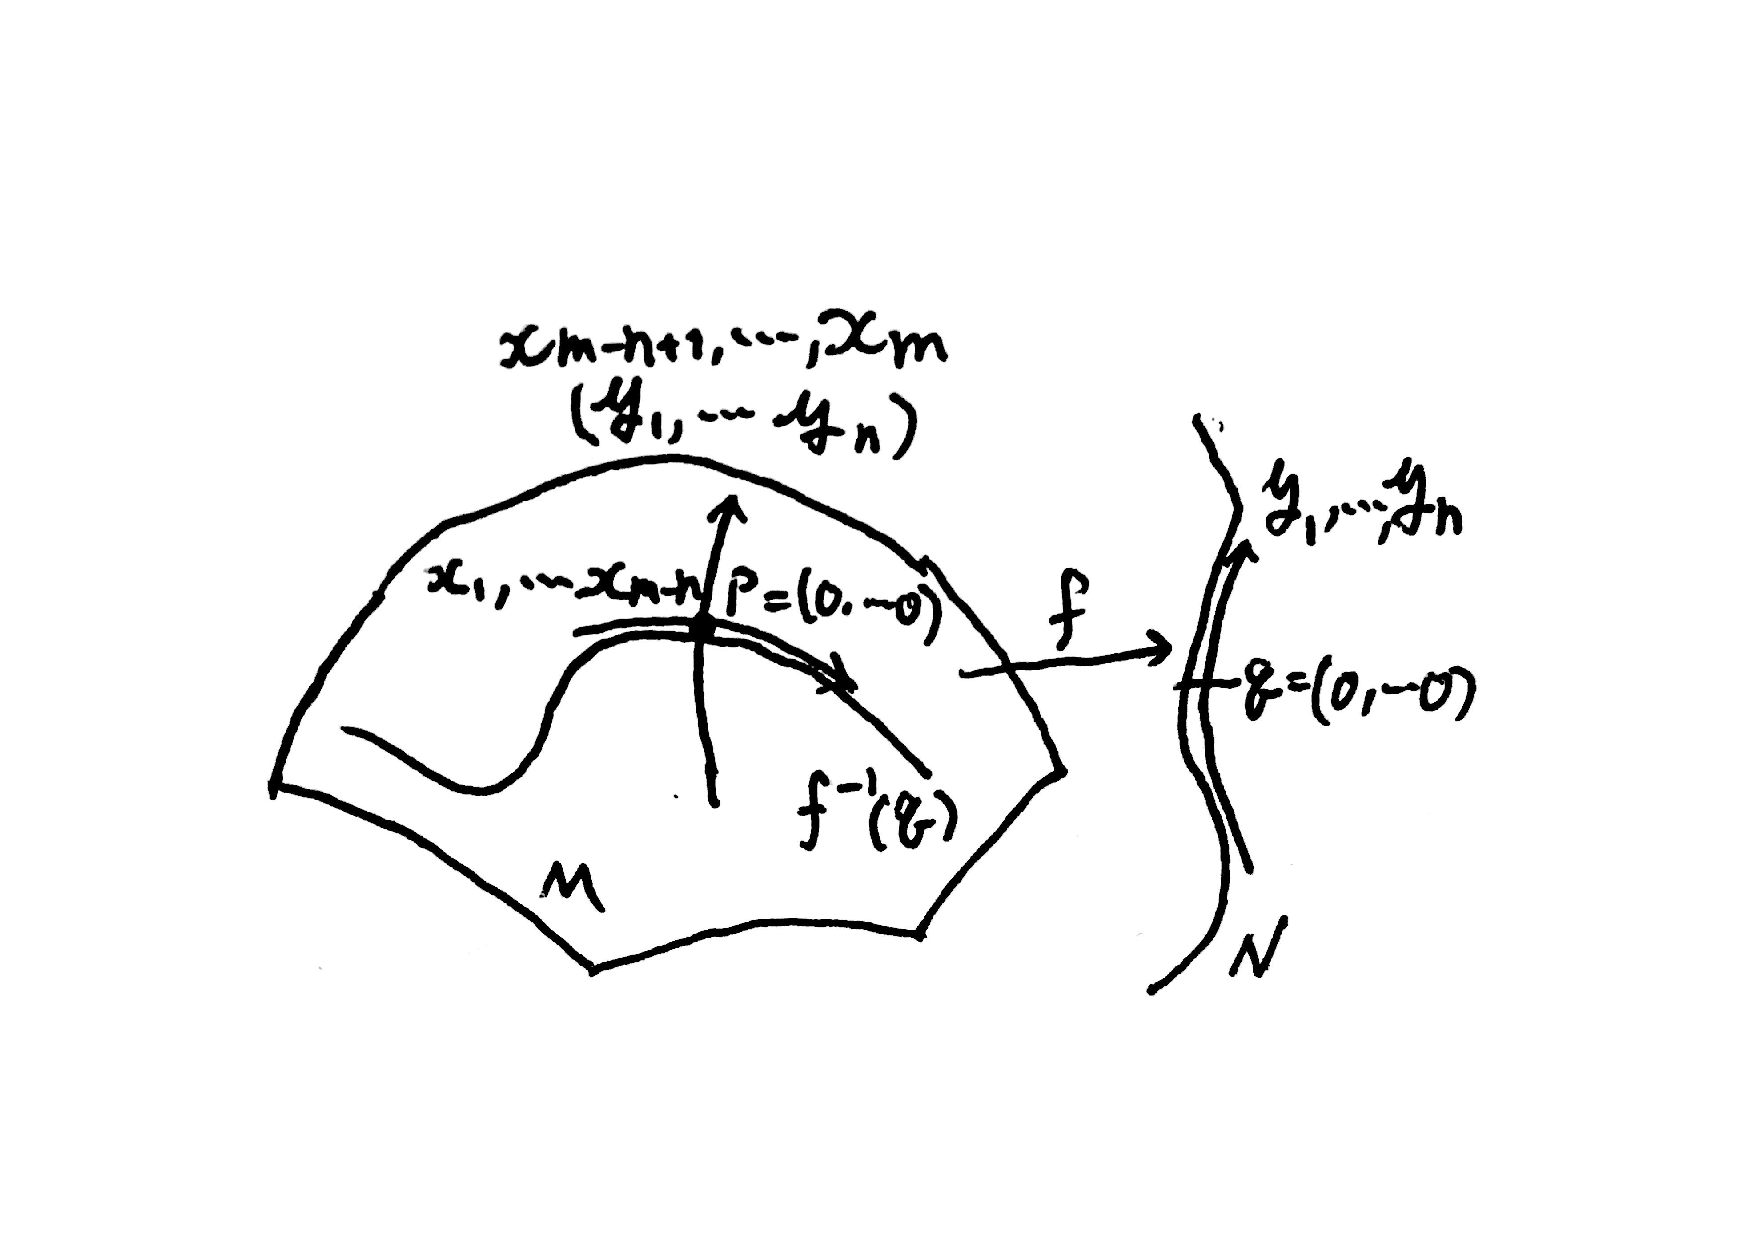
\includegraphics[keepaspectratio, scale=0.35]{finverseIsManifold.pdf}
      \caption{}
      \label{finverseIsManifold}
     \end{figure}
\end{frame}

\section{多様体の次元の具体的な計算}
\begin{frame}
  \frametitle{多様体の次元の具体的な計算}
  \begin{ex}
    $n$次元球面
    $$S^n=\{(x_1,\cdots ,x_{n+1}\in 
    \mathbb{R}^{n+1})|x_1^2+\cdots +x_{n+1}^2=1\}$$
    は$n$次元$C^\infty$級多様体である. 
\end{ex}
$C^\infty$級写像($C^\infty$級関数)
$f:\mathbb{R}^{n+1}\to \mathbb{R}$を
$$f(x_1,\cdots ,x_{n+1})=
x_1^2+\cdots +x_{n+1}^2-1$$
で定義すると, 
$S^n=\{(x_1,\cdots ,x_{n+1}\in 
\mathbb{R}^{n+1})|f(x_1,\cdots ,x_{n+1})=0\}
=f^{-1}(0)$
より, $S^n$は逆像$f^{-1}(0)$となっている. 
ヤコビ行列$(Jf)_{\boldsymbol{x}}$を調べると, 
$\boldsymbol{x}\in S^1$のとき, 
$$(Jf)_{\boldsymbol{x}}=(2x_1,\cdots ,2x_{n+1})
\neq \boldsymbol{o}$$
となり, $(Jf)_{\boldsymbol{x}}$の階数は$1$となる. 
よって, $S^n$は$(n+1)-1=n$次元$C^\infty$級
多様体である. 
\end{frame}

\begin{frame}
  \frametitle{}
  \begin{ex}
    $2$次元トーラス
    $$T^2=S^1\times S^1=
    \{T^2=(x,y,z)\in \mathbb{R}^3|
    (\sqrt{x^2+y^2}-R)^2+z^2=r^2\} $$
    $(0<r<R)$は$2$次元$C^\infty$級多様体である. 
    \begin{figure}[H]
      \centering
      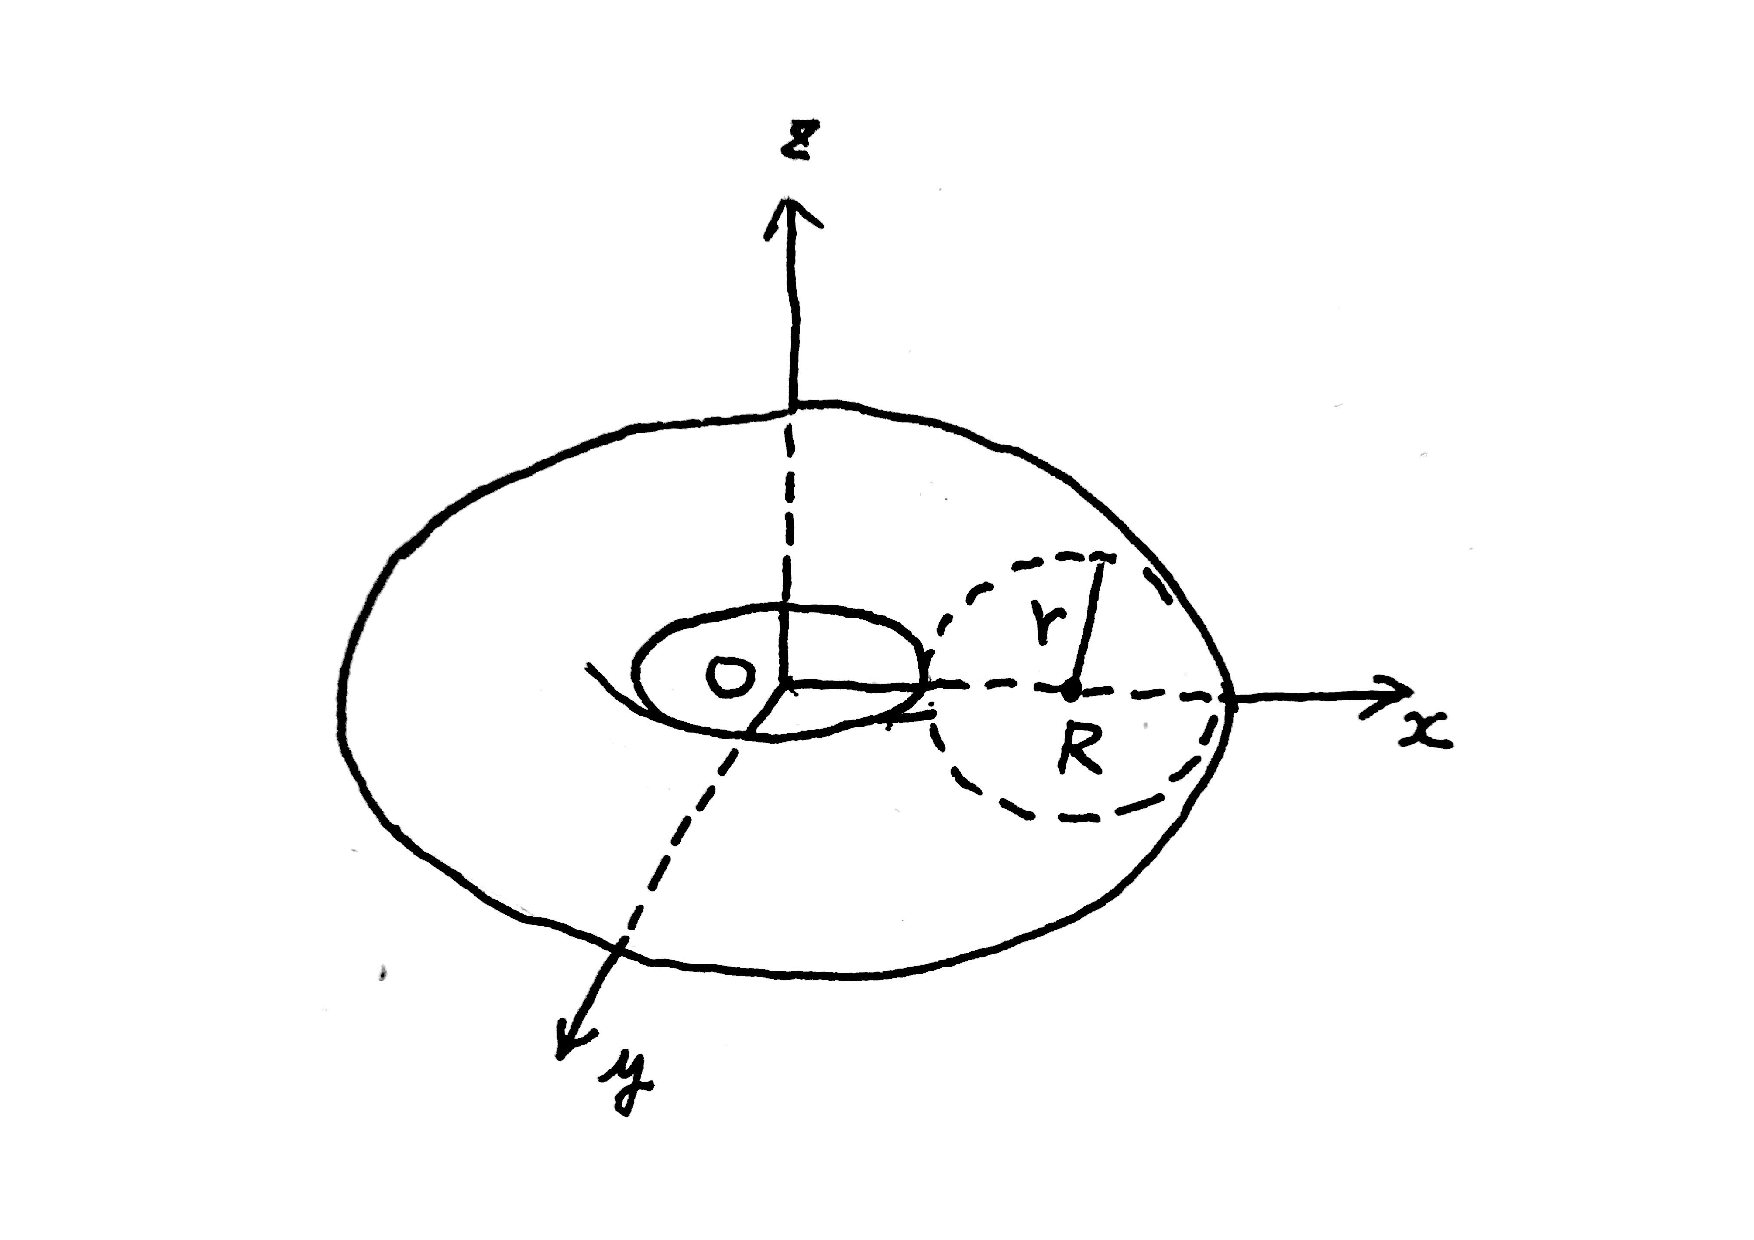
\includegraphics[keepaspectratio, scale=0.2]{T2Noshadow.pdf}
      \caption{$\mathbb{R}^3$の
      中の$2$次元トーラス$T^2$}
      \label{T2Noshadow}
     \end{figure}
\end{ex}
\end{frame}

\begin{frame}
    $C^\infty$級写像($C^\infty$級関数)
    $f:\mathbb{R}^3\to \mathbb{R}$
    を
    $$f(x,y,z)=(\sqrt{x^2+y^2}-R)^2+z^2-r^2$$
    と定義すると, 
    $$T^2=f^{-1}(0)$$
    となる. $\boldsymbol{p}=(x,y,z)$における
    ヤコビ行列
    $(Jf)_{\boldsymbol{p}}$を調べると, 
    であり, $\boldsymbol{p}\in T^2$のとき, 
    $$(Jf)_{\boldsymbol{p}}=
    \left(\frac{2x(\sqrt{x^2+y^2}-R)}
        {\sqrt{x^2+y^2}},\frac{2y(\sqrt{x^2+y^2}-R)}
        {\sqrt{x^2+y^2}},2z\right)\neq 
        \boldsymbol{o}$$
    となり, rank$(Jf)_{\boldsymbol{p}}=1$
    を得る. 
    したがって, $T^2$は$3-1=2$次元$C^\infty$
    級多様体である. 
\end{frame}

\begin{frame}
  \begin{ex}
    $2$次元トーラス$T^2=S^1\times S^1$は
    $2$次元$C^\infty$級多様体になる.  
  \end{ex}  
  $T^2=\{(x_1,x_2,x_3,x_4)\in \mathbb{R}^4|
  x_1^2+x_2^2=1, x_3^2+x_4^2=1\}$
  より, 
  $C^\infty$級写像$f:\mathbb{R}^4\to \mathbb{R}^2$
  を$f(x_1,x_2,x_3,x_4)=(x_1^2+x_2^2-1,
  x_3^2+x_4^2-1)$と定義すると, 
  $T^2=f^{-1}(0,0)$
  と表せる. ヤコビ行列$(Jf)_{\boldsymbol{x}}$は
  $$(Jf)_{\boldsymbol{x}}=
      \left(\begin{array}{cccc}
          2x_1&2x_2&0&0\\
          0&0&2x_3&2x_4
      \end{array}\right)$$
  $\boldsymbol{x}\in T^2$のとき, 
  rank$(Jf)_{\boldsymbol{x}}=2$であるから, 
  $T^2$は$4-2=2$次元$C^\infty$級
  多様体である.
\end{frame}

\begin{frame}
    \frametitle{おわりに}
  空間を多様体$M$, $N$の間の$C^r$級写像$f:M\to N$の逆像$f^{-1}(q)$
(ただし$q$は$N$のある$1$点)
とみなせれば, $f$のヤコビ行列の階数を計算することで
多様体としての次元を調べることができるという
ことが分かった. 

今後の課題としては, 多様体が
部分多様体として実現できる空間の
条件(埋め込み可能性)について調べたい. 
\end{frame}

\begin{frame}
\frametitle{参考文献} 
\begin{thebibliography}{1}
\beamertemplatetextbibitems
\bibitem{Matsumoto18} 松本幸夫, [第30版]多様体の基礎, 東京大学出版会, 2018.
  \bibitem{Hujioka17} 藤岡敦, [第2版]具体例から学ぶ 多様体, 裳華房, 2017.
  \bibitem{Hattori76} 服部晶夫, [第1版]多様体, 岩波書店, 1976.
\end{thebibliography}
\end{frame}

%ここからは補足
\begin{frame}
  \frametitle{}
  \begin{prop}
    連続写像$f:M\to N$が$1$点$p\in M$において
    $C^s$級であるという性質は, $p$, $f(p)$を
    それぞれ含む$C^r$級座標近傍$(U,\varphi)$, 
    $(V, \psi)$の選び方によらない. 
    (ただし, $0\leq s \leq r \leq \infty$)
  \end{prop}
    $f$は$p\in M$において$(U,\varphi)$, 
    $(V, \psi)$に関して$C^s$級であると仮定する. 
    $f(U')\subset V'$, $U'=U$, $V'=V$となるような
    $p$, $f(p)$をそれぞれ含む別の$C^r$級座標近傍
    $(U',\varphi')$, $(V, \psi')$をとると, 
    $\psi'\circ f\circ \varphi'^{-1}$は
    $$\psi'\circ f\circ \varphi'^{-1}=
    (\psi'\circ \psi^{-1})\circ
    (\psi \circ f\circ \varphi^{-1})\circ
    (\varphi \circ \varphi')$$
    と分解される. $\psi'\circ \psi^{-1}$, 
    $\varphi \circ \varphi'$はそれぞれ$M$, $N$
    における座標変換であるから$C^r$級であり, 
    $\psi \circ f\circ \varphi^{-1}$は
    仮定より$C^s$級であるから, 
    $\psi'\circ f\circ \varphi'^{-1}$は
    $C^s$級である. 
\end{frame}

\begin{frame}
  \frametitle{}
  \begin{prop}\label{prop:dim of C^r-submanifold}
    $n$次元$C^r$級多様体$N$の$l$次元$C^r$級
    部分多様体$L$は, それ自身$l$次元$C^r$級
    多様体である. 
  \end{prop}
  $0\leq l<n$のとき, 点$p\in L$に対し, $p$を含む$N$の
  局所座標系で部分多様体の定義の条件を満たすもの
  を選び, $(U_p;x^p_1,\cdots ,x^p_n)$, 
  $(U_q;x^q_1,\cdots ,x^q_n)$とし,  
  $V_p=L\cap U_p$, $V_q=L\cap U_q$とおく.  
  $U_p$, $U_q$の間の座標変換はある$C^r$級関数$f$を
  用いて, 
  %$V_p\cap V_q$上では, 
  % $x^q_{l+1}=\cdots =x^p_n=0$, $x^q_{l+1}=\cdots =x^q_n=0$
  % が成り立つので, $V_p\cap V_q$上では
  \begin{eqnarray*}
      x^q_1&=&f_1(x^p_1, \cdots ,x^p_l,0,\cdots ,0)\\
      &\vdots & \\
      x^q_l&=&f_l(x^p_1, \cdots ,x^p_l,0,\cdots ,0)\\
      0&=&f_{l+1}(x^p_1, \cdots ,x^p_l,0,\cdots ,0)\\
      &\vdots & \\
      0&=&f_n(x^p_1, \cdots ,x^p_l,0,\cdots ,0)\\
  \end{eqnarray*}
\end{frame}
\begin{frame}
  \frametitle{}
  改めて関数$g$を
  \begin{eqnarray*}
  g(x^p_1, \cdots ,x^p_l)&=&
  (g_1(x^p_1, \cdots ,x^p_l), \cdots 
  , g_l(x^p_1, \cdots ,x^p_l))\\
  &=&(f_1(x^p_1, \cdots ,x^p_l,0,\cdots ,0), \cdots 
  , f_l(x^p_1, \cdots ,x^p_l,0,\cdots ,0))
  \end{eqnarray*}
  と定義すると, この関数は$C^r$級である. 
  そして, 
  $$(x^\beta_1, \cdots ,x^\beta_l)
  =g(x^\alpha_1, \cdots ,x^\alpha_l)$$
  が$(V_p;x^p_1,\cdots x^p_l)$から
  $(V_q;x^q_1,\cdots x^q_l)$の座標変換を与えている. \\
  ゆえに, $\{(V_p;x^p_1,\cdots ,x^p_l)\}_{p\in L}$
  は$L$の$C^r$級座標近傍になっている. \\
  以上より, $L$は$l$次元$C^r$級多様体である. 
\end{frame}
\begin{frame}
  \frametitle{}
    今, $f(p)=q$を満たす$p\in M$について, 常に
    rank$(Jf)_p=n$であるから, $(df)_p$は上への
    写像である. よって, 
    $q$($=f(p)$)のまわりの座標近傍$(V;y_1,\cdots ,y_n)$
    に対して, 
    $p$のまわりの座標近傍$(U;x_1,\cdots ,x_m)$を
    とってきて
    $$f|U:U\to V,\ (y_1,\cdots ,y_n)=f(x_1,\cdots x_m)
    =(x_{m-n+1},\cdots ,x_m)$$
    とすることができる.  \\
    $(V;y_1,\cdots ,y_n)$は
    点$q$で$y_1=\cdots =y_n=0$となるように
    とっておくと, 
    \begin{eqnarray*}
        f^{-1}(q)\cap U&=& \{p\in U|f(p)=q\}\\
        &=&\{(x_1,\cdots ,x_m)\in U|f(x_1,\cdots x_m)=(0,\cdots ,0)\}\\
        &=&\{(x_1,\cdots ,x_m)\in U|(x_{m-n+1},\cdots x_m)=(0,\cdots ,0)\}\\
        &=&\{(x_1,\cdots x_m)\in U|x_{m-n+1}=\cdots =x_m=0\}
    \end{eqnarray*}
    となり, 条件を満たす$U$が存在することがわかる. 
\end{frame}
\end{document}